\documentclass[12pt,letterpaper]{article}     % Tipo de documento y otras especificaciones
\usepackage[utf8]{inputenc}                   % Para escribir tildes y eñes
\usepackage[spanish]{babel}                   % Para que los títulos de figuras, tablas y otros estén en español
\addto\captionsspanish{\renewcommand{\tablename}{Tabla}}					% Cambiar nombre a tablas
\addto\captionsspanish{\renewcommand{\listtablename}{Índice de tablas}}		% Cambiar nombre a lista de tablas
\usepackage{geometry}                         
\geometry{left=18mm,right=18mm,top=21mm,bottom=21mm} % Tamaño del área de escritura de la página
\usepackage{ucs}
\usepackage{amsmath}      % Los paquetes ams son desarrollados por la American Mathematical Society
\usepackage{amsfonts}     % y mejoran la escritura de fórmulas y símbolos matemáticos.
\usepackage{amssymb}
\usepackage{graphicx}     % Para insertar gráficas
\usepackage[lofdepth,lotdepth]{subfig}	% Para colocar varias figuras
\usepackage{unitsdef}	  % Para la presentación correcta de unidades
\usepackage{pdfpages}   %incluir paginas de pdf externo, para los anexos
\usepackage{appendix}   %para los anexos
\renewcommand{\unitvaluesep}{\hspace*{4pt}}	% Redimensionamiento del espacio entre magnitud y unidad
\usepackage[colorlinks=true,urlcolor=blue,linkcolor=black,citecolor=black]{hyperref}     % Para insertar hipervínculos y marcadores
\usepackage{float}		% Para ubicar las tablas y figuras justo después del texto
\usepackage{booktabs}	% Para hacer tablas más estilizadas
\usepackage{color}
\batchmode
%\bibliographystyle{plain} 
\pagestyle{plain} 
\pagenumbering{arabic}
\usepackage{lastpage}
\usepackage{fancyhdr}	% Para manejar los encabezados y pies de página
\usepackage{mdframed}
\pagestyle{fancy}		% Contenido de los encabezados y pies de pagina
\setlength{\headheight}{15pt}
\usepackage{multicol}   % Para varias columnas
\usepackage[export]{adjustbox}
\usepackage{ragged2e}
\usepackage{tikz}
\usepackage{pgfplots}
\usepackage{circuitikz}
\usepackage{cancel}
\usepackage{color}
\usepackage{listings}
\lstset{ %
language=C++,                % choose the language of the code
basicstyle=\footnotesize,       % the size of the fonts that are used for the code
numbers=left,                   % where to put the line-numbers
numberstyle=\footnotesize,      % the size of the fonts that are used for the line-numbers
stepnumber=1,                   % the step between two line-numbers. If it is 1 each line will be numbered
numbersep=5pt,                  % how far the line-numbers are from the code
backgroundcolor=\color{white},  % choose the background color. You must add \usepackage{color}
showspaces=false,               % show spaces adding particular underscores
showstringspaces=false,         % underline spaces within strings
showtabs=false,                 % show tabs within strings adding particular underscores
frame=single,           % adds a frame around the code
tabsize=2,          % sets default tabsize to 2 spaces
captionpos=b,           % sets the caption-position to bottom
breaklines=true,        % sets automatic line breaking
breakatwhitespace=false,    % sets if automatic breaks should only happen at whitespace
escapeinside={\%*}{*)}          % if you want to add a comment within your code
}
%%%%
%---------------------------Definición del environment resumen---------------------------
\newcounter{resumen}
\setcounter{resumen}{0}
\def\theejemplo{\thechapter.\arabic{resumen}}

\newenvironment{resumen}
{	
	\begin{center}
	\begin{minipage}[t]{500 pt}
	\vspace{5mm}
	\emph{\textbf{Resumen}}
	\\[-2mm]
	\line(1,0){500}
	\\[-4.25 mm]
	\line(1,0){500}
	\vspace{\baselineskip}
}
{
	\normalsize
	\\[2mm]
	\footnotesize\textbf{Palabras clave: \footnotesize\@palabras}
	\\[-2mm]
	\line(1,0){500}
	\\[0.5cm]
	\end{minipage}
	\end{center}
}

% -------------------- Para las palabras clave -------------- %
\def\palabras#1{\gdef\@palabras{#1}}

%---------------------------Definición del float circuito---------------------------
\newfloat{circuito}{thp}{lop}
\floatname{circuito}{Circuito}

%---------------------------Definición del float código---------------------------
\newfloat{codigo}{thp}{lop}
\floatname{codigo}{Código}

%%%%%%%%%%%%%%%%%%%%%%%%%%%%%%%%%%%%

\lhead{B5692 - Plataforma de programación y prueba para PCB}
\chead{}
\rhead{Desarrollo de maqueta y HMI}	% Aquí va el numero de experimento, al igual que en el titulo
\lfoot{Ingeniería Electrónica}
\cfoot{\thepage\ de \pageref{LastPage}}
\rfoot{Universidad Nacional de Río Negro}

%%%%%%%%%%%%%%%%% PALABRAS CLAVE 
\palabras{Punto de trabajo, pequeña señal, analíticamente, simulación, laboratorio}
%%%%%%%%%%%%%%%%%
% Se escriben después del resumen y sintetizan los conceptos fundamentales del experimento a modo de etiquetas


%%%%%%%%%%%%%%%%
\begin{document}	% Inicio del documento
%%%%%%%%%%%%%%%%
\pdfbookmark[1]{Portada}{portada} 	% Marcador para el título

\begin{titlepage}
\centering
{
\includegraphics[width=0.2\textwidth]{imagenes/LOGOUNRN.jpg}\par}
\vspace{0.5cm}
{\bfseries\large Universidad Nacional de Río Negro \par}
\vspace{0.5cm}
{\scshape\large Escuela de Producción, Tecnología y Medio Ambiente \par}
\vspace{0.5cm}
{\scshape\large Ingeniería Electrónica \par}
\vspace{3cm}
{\bfseries\Large Plataforma de programación y prueba para PCB \par}
{\Large Desarrollo de maqueta y HMI\par}
\vfill
{\large \textbf{Alumno:} Mirko Manuel Pojmaevich\par}
{\large \textbf{Profesores:} Gelardi Gustavo\par}
{\large \textbf{Materia:} Electrónica Analógica | \textbf{Código:} B5692\par}
\vspace{3cm}
{\large Fecha de entrega: 10 de noviembre de 2022 \par}
\vspace{1cm}
\begin{table*}[!ht]
\begin{center}
\begin{tabular}{| c | c | c | c |}
\hline
\textbf{Rev.} & \textbf{Fecha} & \textbf{Profesor} & \textbf{Nota} \\ 
\hline
 &  & & \\
 \hline
 & & &  \\
\hline
\end{tabular}
\end{center}
\end{table*}
\end{titlepage}
%\maketitle							% Título
\newpage
\tableofcontents
\newpage
\listoffigures
%\listoftables

\newpage
%palabras claves
\section{Resumen}
%%%%%%%%%%%%%%%%%%%
\begin{resumen}
	Se presenta un sistema automático para la validación de circuitos electrónicos.
	Este inyecta señales en la placa siendo probada y mide las señales de respuesta.
	Es capaz de medir tanto señales digitales como niveles analógicos de tensión.
	Para circuitos que incluyen un microcontrolador, de tipo PIC, el sistema es capaz de programar
	firmware, permitiendo probar la correcta funcionalidad de los módulos internos
	del dispositivo. El sistema clasifica los circuitos probados separando los
	funcionales de los defectuosos de acuerdo al conjunto de reglas que se le den.
	El estado de las pruebas puede ser monitoreado mediante un HMI.
\end{resumen} 
%%%%%%%%%%%%%%%%%%% 
%\section{Objetivos} 
% 
%\begin{itemize} 
%\item Aplicar mediante un ejemplo práctico conocimientos vistos en la materia.
%\item Ampliar conocimientos y herramientas referidas a filtros.
%\end{itemize}
%\newpage
%%%%%%%%%%%%%%%%%%%%%%%%%%%%%%%%%%
\section{Marco teórico}
\label{Marco teórico}

\subsection{Pogopins}

Se conoce como Pogopin a un tipo de contacto con muelle como el que se muestra en la figura \ref{fig:pogopin}.
Este permite realizar una conexión con una circuito impreso con únicamente un pad expuesto de forma robotizada.

\begin{figure}[!ht]
\centering
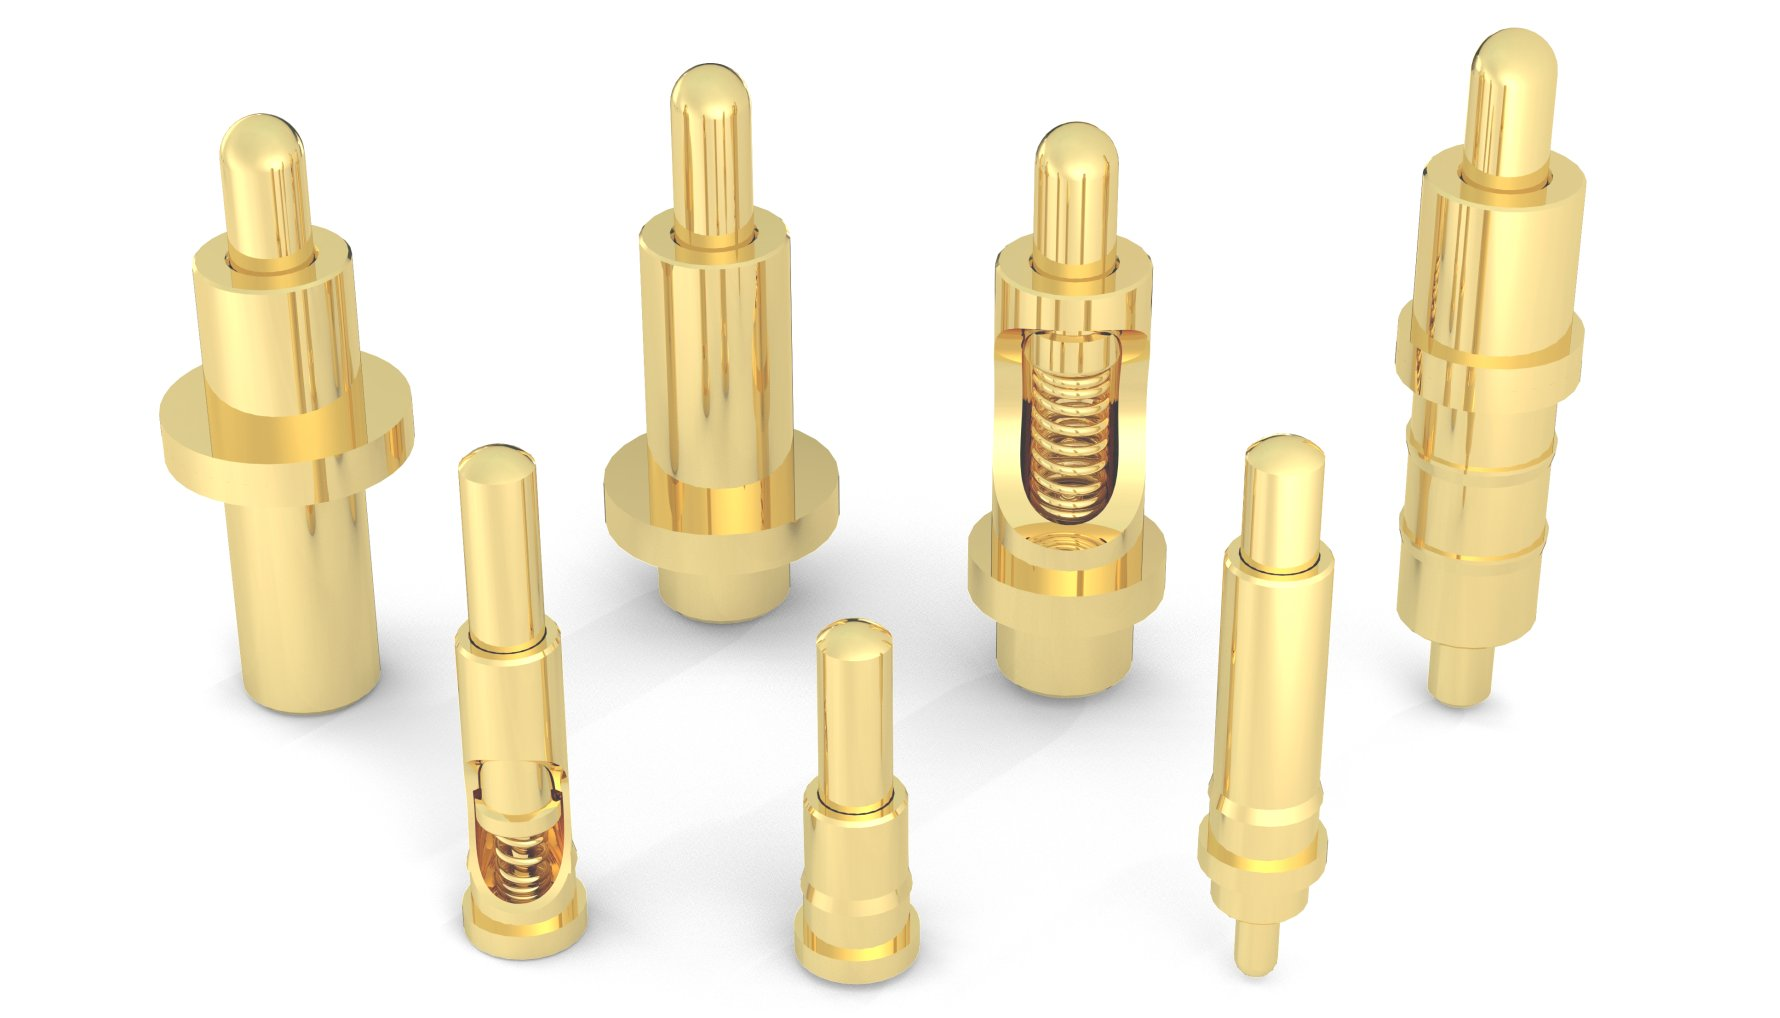
\includegraphics[]{imagenes/pogopin.jpg}
\caption{Ejemplo de Pogopins}
\label{fig:pogopin}
\end{figure}

\subsection{SBC}

SCB son las siglas en ingles de Single Board Computer, refieren a una computadora completamente contenida en una
única placa de circuito impreso. El ejemplo mas popular son las RaspberryPi.

\subsection{/dev}

En el sistema de directorios de Linux el directorio /dev es uno que contiene archivos especiales 
o de tipo dispositivo. En su mayoría los archivos contenidos en este directorio permiten interactuar con el
hardware, tratando a los dispositivos físicos del sistema como parte del sistema de ficheros. Esto funciona 
asociando los canales de lectura y escritura de los archivos con los dispositivos físicos. Por ejemplo
si se escribe al archivo /dev/dsp, el cual representa los parlantes, se escuchará un sonido. Para el correcto
funcionamiento de los dispositivos se debe respetar el protocolo mediante el cual se interactua con estos archivos.

\subsubsection{Módulos del kernel}

No todos los archivos bajo /dev representan un dispositivo, algunos representan extensiones del kernel de Linux.
Estas extensiones generalmente interactúan con uno o mas dispositivos físicos bajo un protocolo distinto, esto

existe una extensión de kernel para el manejo de LCDs, estos podrían ser controlados mediante escritura a los
ficheros de entrada y salida, o algún fichero de un modulo de comunicación serie, en ambos casos los que se 
escribe en los archivos de /dev no es lo que se desea obtener, sino que se debe "traducir" el mensaje mediante el
software y realizar múltiples llamados al sistema desde el entorno de usuario para la escritura. En el caso de un
modulo de kernel dedicado, se puede escribir la información final que se desea obtener y la traducción y envío del
mensaje ocurrirá en espacio del kernel de forma muy eficiente con una única llamada al sistema. 

\clearpage
\section{Materiales}

En esta sección se describen los elemento utilizados para la realización del proyecto, no se discute si la
elección fue optima porque estos son productos de los que se disponía con antelación.

\subsection{NanoPi Neo3}

El NanoPi Neo3 es una SBC compacta y de bajo costo. Utiliza un CPU Rockchip RK3328 de cuatro núcleos, con
arquitectura ARM Cortex-A53. Cuenta con 1 ó 2 GB de memoria RAM, y Gbps Ethernet. 

\begin{figure}[!ht]
\centering
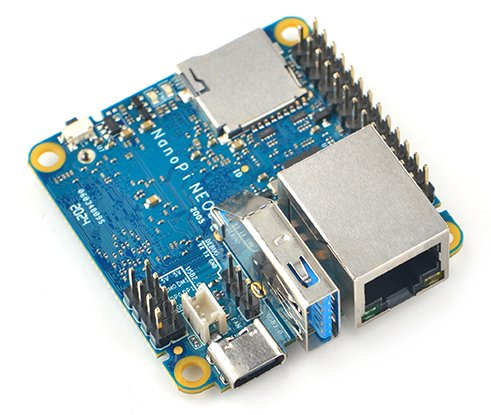
\includegraphics[scale=0.5]{imagenes/naopi.jpg}
\caption{NanoPi Neo3}
\label{fig:pogopin}
\end{figure}

Esta SCB interactúa con los sensores y motores coordinando el funcionamiento de la plataforma.
A su vez esta se encarga de programar los microcontroladores, inyectar las señales, y leer 
las respuestas digitales. Como la mayoría de SCBs no contienen un ADCs incorporado, se utiliza
un dispositivo externo para la medición analógica de niveles de tensión, los que luego son
comunicados mediante le protocolo I2C.

Por ultimo este SCB actúa como host de un servidor TCP, para que múltiples usuarios puedan acceder
al HMI de forma remota.

\subsection{PIC18F45K50}

Este microcontrolador es el dispositivo externo antes mencionado que actúa como ADC y comunica los
valores de tensión medidos mediante I2C. Este resulta mucho mas capaz de lo requerido para la tarea.

\subsection{Motorreductor}

Para movilizar la cinta se utiliza un motor con una reducción 1:48 y salida en doble eje TT de marca
genérica similar al que se muestra en la figura \ref{fig:motor}.

\begin{figure}[!ht]
\centering
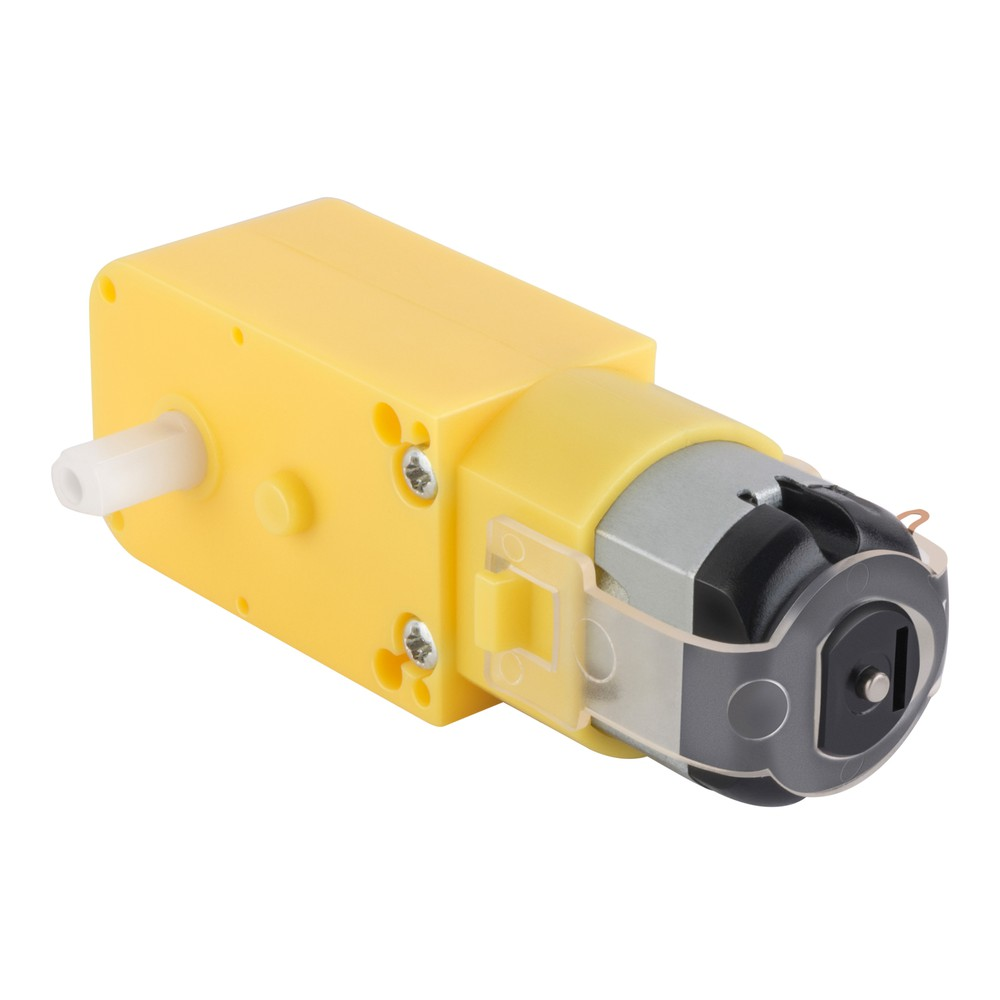
\includegraphics[scale=0.25]{imagenes/motorreductor.jpg}
\caption{Motorreductor}
\label{fig:motor}
\end{figure}

\subsection{Servo motor}

Los servo motores utilizados son micro servos, modelo MG90S, de la marca Tower Pro, como el que
se muestra en la figura \ref{fig:servo}. Este cuenta con un torque de $1,8\kilogram f$ a $4,8\volt$,
y $2,2\kilogram f$ a $6\volt$.

\begin{figure}[!ht]
\centering
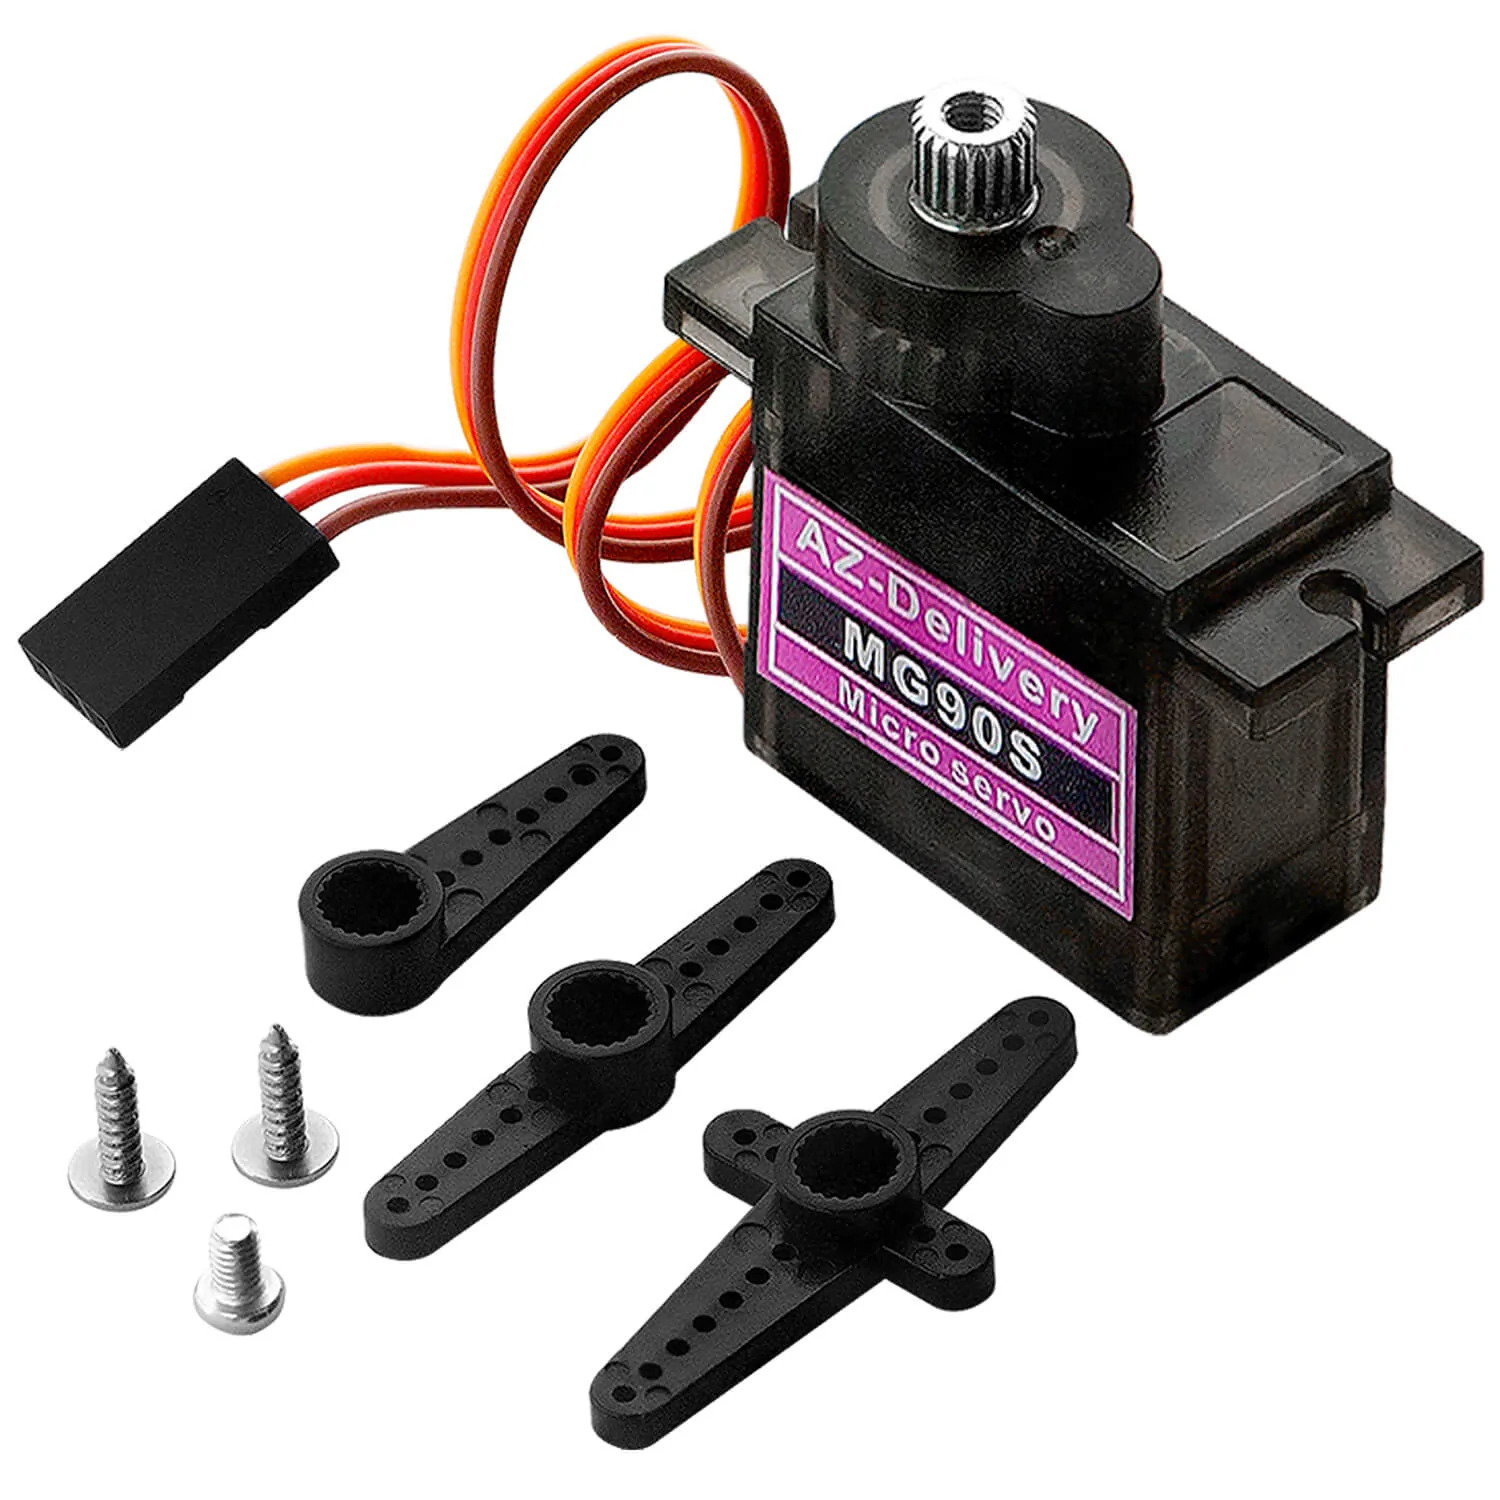
\includegraphics[scale=0.15]{imagenes/servo.jpg}
\caption{Servo motor}
\label{fig:servo}
\end{figure}

\subsection{Sensor óptico}

Para detectar la presencia de una placa en los puntos relevantes del proceso se utilizaron sensores ópticos.
Estos consisten de un led y un fototransistor, dispuestos de manera tal que el led permita que el fototransistor
sature, la detección ocurre cuando un objeto obstruye el paso de luz, causando que le fototransistor entre en
corte. Su aspecto y diagrama esquemático se pueden ve en la figura \ref{fig:sensoptico}.

\begin{figure}[!h]
	\begin{minipage}{.5\textwidth}
		\begin{center}
			\begin{circuitikz}[american,]
				\draw (0,0) node[npn, photo](Q1){};
				\draw (Q1.E) to[short]
					++(0,0)
					to[short]
					++(-2,0)
					node[](gnd){};
				\draw (Q1.C) to [short, -o] 
					++(1.5, 0)
					node[](out){};
				\draw (-2,0.6) 
					to[leD]
					++(0,-1)
					to[short]
					(gnd |- gnd);
				\draw (-2,0.6)
					to[short]
					(gnd |- out)
					to[short, -o]
					++(-1.5,0);
				\draw (-1,-0.77)
					to[short, *-o]
					++(0,-1);
			\end{circuitikz}
		\end{center}
	\end{minipage}%
	\begin{minipage}{.5\textwidth}
		\begin{center}
			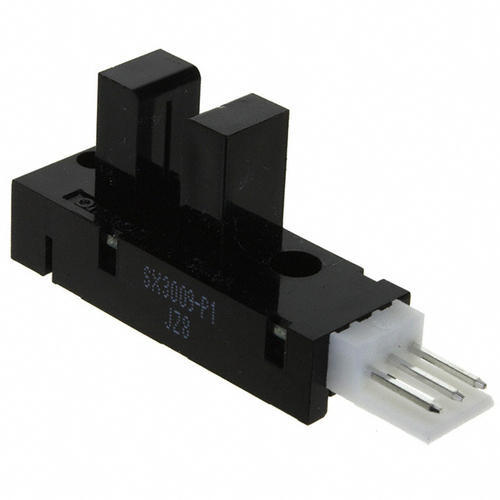
\includegraphics[scale=0.3]{imagenes/optico.jpg}
		\end{center}
	\end{minipage}
\caption{Sensor óptico}
\label{fig:sensoptico}
\end{figure}

\subsection{Pickle}

Para poder realizar la programación de los PIC se utiliza el software Pickle. 
Este provee una mecanismo para interactuar con el microcontrolador y quemar en el firmware.
Su instalación es sencilla y puede lograrse con los comandos mostrados en el Código \ref{code:instalacionPickle}.
Sin embargo, este solo posee soporte nativo para una contada selección de SBCs populares. En el caso del NanoPi NEO3,
el programa depende de un modulo externo del kernel de Linux llamado GPIO BIT BANG.
Compilar módulos del kernel requiere de la instalación de los headers del kernel, los cuales están asociados al kernel
que se tiene instalado, el que a su vez depende de la arquitectura en la que se trabaje. Los paquetes de headers en los
repositorios de Linux suelen seguir un consenso en sus nombres, bajo la siguiente estructura, 
$linux-headers-\$(uname -r)$. En el caso del NanoPi NEO3, este consenso se rompe siendo el nombre del paquete, 
$linux-headers-current-rockchip64$. Una vez instalados los headers del kernel, uno debe asegurarse de que exista
un enlace simbólico, del directorio $/lib/modules/\$(uname -r)/build$ al directorio $/usr/src/$.
Una vez todas las herramientas para la extensión del kernel estén en su lugar, se puede instalar el modulo 
GPIO BIT BANG mediante los comandos mostrados en el Código \ref{code:instalacionGPIOBB} (el comando $hg$ requiere
de la instalación de mercurial).

\begin{codigo}[]
	\begin{lstlisting}
	cd /tmp
	wget http://wiki.kewl.org/downloads/pickle-4.20.tgz 
	tar zxf pickle-4.20.tgz 
	cd pickle-4.20/
	make
	sudo make install
	\end{lstlisting}
	\caption{Instalación Pickle}robotizada
Cómo se pronuncia
	\label{code:instalacionPickle}
\end{codigo}

\begin{codigo}[!h]
	\begin{lstlisting}
	hg clone http://hg.kewl.org/pub/gpio-bb
	cd gpio-bb
	make
	sudo make install
	\end{lstlisting}
	\caption{Instalación GPIO BIT BANG}
	\label{code:instalacionGPIOBB}
\end{codigo}



\newpage
\section{Ejercicios}
\begin{mdframed}
	\begin{itemize}
		\item Análisis en CC
		\begin{enumerate}
			\item Busque la hoja de datos del transistor BC547 y obtenga los siguientes valores:
			\begin{itemize}
				\item Ganancia de corriente ($h_{fe}$)
				\item Tensión base-emisor de encendido ($V_{BE}$)
				\item Tensión colector-emisor máxima ($V_{CEmax}$)
				\item Tensión colector-emisor de saturación ($V_{CEsat}$)
				\item Corriente de colector máxima
			\end{itemize}
			\item Con los datos obtenidos, resuelva el circuito que se muestra en la figura \ref{circuito1} 
				analíticamente para CC ($V_{in}=0$). Halle el punto de trabajo y grafíquelo.
			\item Simúlelo y obtenga el punto de trabajo mediante simulación. Compare con lo calculado analíticamente.
		\end{enumerate}
		\item Análisis en CA
		\begin{enumerate}
			\item Resuelva el circuito \ref{circuito2} analíticamente para CA
			\item Simúlelo y compare con los resultados obtenidos analíticamente.
			\item ¿Qué diferencia se presentaría de utilizar un capacitor de desacople para $R_3$?
		\end{enumerate}
		\item Laboratorio
		\begin{enumerate}
			\item Implemente el circuito \ref{circuito2} en protoboard y registre la señal en función de la
				señal de la entrada. Modifique la señal de entrada en un $20\%$ y registre el
				cambio de la salida correspondiente. Obtenga a partir de la gráfica el valor
				de $A_V$. (Recuerde que la mayoría de los osciloscopios modernos permiten
				guardar la forma de onda en un dispositivo USB).
			\item Mida $V_{CE}$ e $I_C$ (Si se le dificulta la medición de corriente recuerde 
				que puede calcularlo mediante la medición de $V_{R1}$ y $R_1$)..
		\end{enumerate}
	\end{itemize}
\end{mdframed}

\begin{circuito}[!h]
	\begin{minipage}{.5\textwidth}
		\begin{center}
			\begin{circuitikz}[american,]
				\draw (0,0) node[npn](Q1){$Q_1$};
				\draw (Q1.E) to[R=$R_3$]
				++(0,-3) node[ground](GND){};
				\draw (Q1.C) to[R=$R_1$]
					++(0,3) node[vcc](VCC){$V_{CC}$};
				\draw (Q1.B) to [short] 
					++(-1,0) node[](in){} 
					to[R=$R_4$]
					(in |- GND) node[ground](){};
				\draw (in |- in) to [R=$R_2$, *-] 
					(in |- VCC) node[vcc](){$V_{CC}$};
				\draw (in) ++(0.1,0) to [short, -o] 
					++(-1.5, 0);
				\draw (Q1.C) to [short, *-o] 
					++(1.5, 0);
			\end{circuitikz}
		\end{center}
	\end{minipage}%
	\begin{minipage}{.5\textwidth}
		\begin{center}
			\begin{tabular}{| c | c |}
				\hline
				$Q_1$&BC547\\
				\hline
				$R_1$&$10\kiloohm$\\
				\hline
				$R_2$&$100\kiloohm$\\
				\hline
				$R_3$&$1\kiloohm$\\
				\hline
				$R_4$&$10\kiloohm$\\
				\hline
				$V_{CC}$&$12\volt$\\
				\hline
			\end{tabular}
		\end{center}
	\end{minipage}
\caption{}
\label{circuito1}
\end{circuito}


\begin{circuito}[!h]
	\begin{minipage}{.5\textwidth}
		\begin{center}
			\begin{circuitikz}[american,]
				\draw (0,0) node[npn](Q1){$Q_1$};
				\draw (Q1.E) to[R=$R_3$]
				++(0,-3) node[ground](GND){};
				\draw (Q1.C) to[R=$R_1$]
					++(0,3) node[vcc](VCC){$V_{CC}$};
				\draw (Q1.B) to [short] 
					++(-1,0) node[](in){} 
					to[R=$R_4$]
					(in |- GND) node[ground](){};
				\draw (in |- in) to [R=$R_2$, *-] 
					(in |- VCC) node[vcc](){$V_{CC}$};
				\draw (in) ++(0.1,0) to[C=$C_2$] 
					++(-3, 0) node[](supl){}
					to[sV=$V_{in}$]
					(supl |- GND) 
					node[ground](){};
				\draw (Q1.C) to[C=$C_1$, *-] 
					++(3, 0) node[](out){}
					to[R=$R_5$]
					(out |- GND) node[ground](){};
			\end{circuitikz}
		\end{center}
	\end{minipage}%
	\begin{minipage}{.5\textwidth}
		\begin{center}
			\begin{tabular}{| c | c |}
				\hline
				$Q_1$&BC547\\
				\hline
				$R_1$&$10\kiloohm$\\
				\hline
				$R_2$&$100\kiloohm$\\
				\hline
				$R_3$&$1\kiloohm$\\
				\hline
				$R_4$&$10\kiloohm$\\
				\hline
				$R_5$&$10\kiloohm$\\
				\hline
				$C_1$&$1\microfarad$\\
				\hline
				$C_2$&$1\microfarad$\\
				\hline
				$V_{CC}$&$12\volt$\\
				\hline
				$V_{in}$&$1{\volt}_{pp}$,5kHz\\
				\hline
			\end{tabular}
		\end{center}
	\end{minipage}
\caption{}
\label{circuito2}
\end{circuito}

\clearpage
\section{Análisis en CC}

\subsection{}
Los valores obtenidos de la hoja de datos son:

\begin{table}[!ht]
	\begin{center}
		\begin{tabular}{| c | c | c |}
			\hline
			\textbf{Parámetro} & \textbf{Valor} & \textbf{Unidad}\\ 
			\hline
			{Ganancia de corriente ($h_{fe}$} & {450/600/900} & {$\beta$/420/520/800}\\
			\hline
			{Tensión base-emisor máxima ($V_{BE}$)} & {0,7} & {$\volt$}\\
			\hline
			{Tensión colector-emisor máxima ($V_{CEmax}$)} & {30} & {${\volt}_{dc}$}\\
			\hline
			{Tensión colector-emisor de saturación ($V_{CEsat}$)} & {0,6} & {$\volt$}\\
			\hline
			{Corriente de colector máxima} & {100} & {${\milliampere}_{dc}$}\\
			\hline
		\end{tabular}
	\end{center}
\caption{Valores obtenidos de la hoja de datos}
\label{tab:tabla1}
\end{table}

\subsection{}

Para el análisis en continua del circuito \ref{circuito1}, comienzo por
calcular la tensión en la base ($V_B$).
Para lograr esto considero un divisor resistivo involucrando a $R_2$, $R_4$
y la impedancia reflejada de $R_3$, que no es mas que $R_3\cdot(\beta+1)$.

\begin{equation}
	\beta=520
\end{equation}

\begin{equation}
	V_B=
	12\volt\cdot\frac{
		10\kiloohm\parallel521\kiloohm
	}{
		100\kiloohm+10\kiloohm\parallel521\kiloohm
	}
\end{equation}

\begin{equation}
	V_B\approx
	12\volt\cdot\frac{
		9,8\kiloohm
	}{
		109,8\kiloohm
	}
\end{equation}

\begin{equation}
	V_B\approx
	1,07\volt
\end{equation}

Conociendo $V_B$ y $V_{BE}$ se puede calcular $I_{BQ}$.

\begin{equation}
	V_B=
	V_{BE}+
	(\beta+1)\cdot
	I_{BQ}\cdot
	1\kiloohm
\end{equation}

\begin{equation}
	1,07\volt\approx
	0,7\volt+
	521\kiloohm\cdot
	I_{BQ}\cdot
\end{equation}

\begin{equation}
	370\millivolt\approx
	521\kiloohm\cdot
	I_{BQ}\cdot
\end{equation}

\begin{equation}
	I_{BQ}\approx
	\frac{
		370\millivolt
	}{
		521\kiloohm\cdot
	}
\end{equation}

\begin{equation}
	I_{BQ}\approx
	710\nanoampere
\end{equation}

\newpage
Sabiendo $I_{BQ}$ se  puede calcular $I_{CQ}$

\begin{equation}
	I_{CQ}=
	\beta\cdot
	I_{BQ}
\end{equation}

\begin{equation}
	I_{CQ}=
	520\cdot
	710\nanoampere
\end{equation}

\begin{equation}
	I_{CQ}=
	369,2\microampere
\end{equation}

Sabiendo $I_{CQ}$ podemos calcular $V_C$.

\begin{equation}
	V_C=
	VCC-
	10\kiloohm\cdot
	I_{CQ}
\end{equation}

\begin{equation}
	V_C=
	12\volt-
	10\kiloohm\cdot
	369,2\microampere
\end{equation}

\begin{equation}
	V_C=
	8,308\volt
\end{equation}

Ahora debemos calcular $V_E$ para así poder calcular $V_{CE}$.

\begin{equation}
	V_E=
	(\beta+1)\cdot
	I_{BQ}\cdot
	1\kiloohm
\end{equation}

\begin{equation}
	V_E=
	369,91\millivolt
\end{equation}

Una vez calculada $V_E$, podemos calcular $V_{CE}$.

\begin{equation}
	V_{CE}=
	V_C-
	V_E
\end{equation}

\begin{equation}
	V_{CE}=
	8,308\volt-
	369,91\millivolt
\end{equation}

\begin{equation}
	V_{CE}=
	7,93809\volt
\end{equation}

De este modo concluimos que el punto de trabajo está dado por:

\begin{table}[!ht]
	\begin{center}
		\begin{tabular}{| c | c | c |}
			\hline
			\textbf{Parámetro} & \textbf{Valor} & \textbf{Unidad}\\ 
			\hline
			{$I_{BQ}$} & {710} & {$\nanoampere$} \\
			\hline
			{$I_{CQ}$} & {369,2} & {$\microampere$}\\
			\hline
			{$V_{CEQ}$} & {7,93809} & {$\volt$}\\
			\hline
		\end{tabular}
	\end{center}
	\caption{Punto de trabajo circuito \ref{circuito1}}
\label{tab:PuntoDeTrabajoCalculo}
\end{table}

\newpage
Este se puede ver graficado en la figura \ref{fig:PuntoQ}.

\begin{figure}[!ht]
	\begin{center}
	\begin{tikzpicture}[
		declare function={
		recta_de_carga(\x)=
		(\x) * (-1.09/12) + 1.09;
		BJT(\x)= 
		0.445 -
		(1.09) * (e^(0.7/(\x+2.05)) - 1);
		}
	]
	\begin{axis}[
		xmin=0, xmax=13,
		ymin=0, ymax=1.3, ytick={0,0.2,...,1.2},
		axis lines=left,
		domain=0:20,
		xlabel = {$V_{CE} [\volt]$},
		ylabel = {$I_{CQ} [\milliampere]$},
		legend style={at={(1.4,1)}},
	]
	\addplot [mark=none,draw=red]  {BJT(x)};
	\addplot [mark=none,draw=blue] {recta_de_carga(x)};
	\addlegendentry{$I_{BQ}=710\nanoampere$}
	\addlegendentry{Recta de carga}
	\end{axis}
	\draw[gray, dashed] (4.18,0) -- (4.18,1.6);
	\draw[gray, dashed] (0,1.6) -- (4.18,1.6);
	\draw[gray, dashed, <-] (4.18,1.8) -- (4.18,3.2) node[anchor=south]{$(7,93809\volt,369,2\microampere)$};
	\filldraw[black] (4.18,1.6) circle (2pt) node[anchor=south west]{Punto Q};
	\end{tikzpicture}
	\caption{Punto de trabajo}
	\label{fig:PuntoQ}
	\end{center}
\end{figure}

\subsection{}

Se simuló el circuito mediante ngspice (usando el modelo siguiente),
los resultados obtenidos se muestran en la tabla \ref{tab:PuntoDeTrabajoSimulado}.

\begin{lstlisting}
.model bc547c NPN BF=730 NE=1.4 ISE=29.5F IKF=80M IS=60F VAF=25 ikr=12m
+ BR=10 NC=2 VAR=10 RB=280 RE=1 RC=40 VJE=.48 tr=.3u tf=.5n
+cje=12p vje=.48 mje=.5 cjc=6p vjc=.7 mjc:.33 isc=47.6p kf=2f
\end{lstlisting}

\begin{table}[!ht]
	\begin{center}
		\begin{tabular}{| c | c | c | c |}
			\hline
			\textbf{Parámetro} & \textbf{Valor calculado} & \textbf{Valor simulado} & \textbf{Unidad}\\ 
			\hline
			{$V_{BQ}$} & {1,07} & {1,08276} & {$\volt$} \\
			\hline
			{$I_{BQ}$} & {710} & {896,134} & {$\nanoampere$} \\
			\hline
			{$I_{CQ}$} & {369,2} & {494,684} & {$\microampere$}\\
			\hline
			{$V_{CQ}$} & {8,308} & {7,05317} & {$\volt$}\\
			\hline
			{$V_{EQ}$} & {369,91} & {495,579} & {$\millivolt$}\\
			\hline
			{$V_{CEQ}$} & {7,93809} & {7,007591} & {$\volt$}\\
			\hline
		\end{tabular}
	\end{center}
	\caption{Punto de trabajo circuito \ref{circuito1}}
\label{tab:PuntoDeTrabajoSimulado}
\end{table}

\clearpage
\section{Análisis en CA}
\subsection{}

Dado que solo tenemos el parámetro híbrido $h_{fe}$, se utiliza el modelo $R_{\pi}$
para el calculo del circuito equivalente.

\begin{equation}
	R_{\pi}=
	\frac{
		h_{fe}\cdot V_T
	}{
		I_{CQ}
	}
\end{equation}

\begin{equation}
	V_T=
	\frac{
		k\cdot T
	}{
		Q
	}
\end{equation}

\begin{equation}
	V_T=
	26\millivolt
	(t=25\degree C)
\end{equation}

\begin{equation}
	h_{fe}=
	600
\end{equation}

\begin{equation}
	I_{CQ}=
	369,2\microampere
\end{equation}

\begin{equation}
	R_{\pi}=
	\frac{
		600\cdot 26\millivolt
	}{
		369,2\microampere
	}
\end{equation}

\begin{equation}
	R_{\pi}=
	42,2535\kiloohm
\end{equation}

\begin{circuito}[!h]
	\begin{minipage}{.7\textwidth}
			\begin{center}
				\begin{circuitikz}[american,]
					\draw (0,0)  node[above](B){B} 
								to[R=$R_4 // R_2$]
						(0,-3) node[ground](GND){};
						\draw (0,0) to[short, i=$i_b$, *-]
						++(1.5,0);
						\draw (0.6,0) to[R=$R_\pi$, -*]
						++(3,0) node[above](){E} 
								node[](E){} 
								to[R=$R_3$] 
						++(0,-3) node[ground](){};
					\draw (B |- E) to[short] 
						++(-2, 0) node[](supl){}
						to[sV=$V_{in}$] (supl |- GND) 
						node[ground](){};
					\draw (E |- E) to[cisource, l=$h_{fe}\cdot i_b$, invert]
						++(3, 0) node[above](C){C}
						to[R=$R_1$]
						(C |- GND) node[ground](){};
					\draw (C |- E) to [short, *-] 
						++(2,0) node[](out){}
						to[R=$R_5$]
						++(0,-3) node[ground](){};
					\draw (out |- out) to [short, *-o] 
						++(1,0) node[right](){$V_{out}$};
				\end{circuitikz}
		\end{center}
	\end{minipage}%
	\begin{minipage}{.3\textwidth}
		\begin{center}
			\begin{tabular}{| c | c |}
				\hline
				$R_1$&$10\kiloohm$\\
				\hline
				$R_2$&$100\kiloohm$\\
				\hline
				$R_3$&$1\kiloohm$\\
				\hline
				$R_4$&$10\kiloohm$\\
				\hline
				$R_5$&$10\kiloohm$\\
				\hline
				$R_{\pi}$&$42,3\kiloohm$\\
				\hline
				$V_{in}$&$1{\volt}_{pp}$,5kHz\\
				\hline
			\end{tabular}
		\end{center}
	\end{minipage}
\caption{Modelo $R_{\pi}$ equivalente al circuito \ref{circuito2}}
\label{circuito3}
\end{circuito}

\newpage
Primero calculo $i_b$.

\begin{equation}
	V_{in}=
	R_{\pi}\cdot 
	i_b +
	(h_{fe}+1) \cdot 
	R_3\cdot
	i_b
\end{equation}

\begin{equation}
	V_{in}=
	i_b\cdot
	[R_{\pi} +
	(h_{fe}+1) \cdot 
	R_3]
\end{equation}

\begin{equation}
	i_b=
	\frac{
		V_{in}
	}{
		R_{\pi} +
		(h_{fe}+1) \cdot 
		R_3
	}
\end{equation}

\begin{equation}
	i_b=
	\frac{
		1\volt_{pp}
	}{
		42,3\kiloohm +
		601\kiloohm
	}
\end{equation}

\begin{equation}
	i_b\approx
	1,554\microampere
\end{equation}

Sabiendo $i_b$ se puede calcular $V_{out}$.

\begin{equation}
	V_{out}=
	-h_{fe}\cdot
	i_b\cdot
	(R_1\parallel
	R_5)
\end{equation}

\begin{equation}
	V_{out}\approx
	-600\cdot
	1,554\microampere\cdot
	(10\kiloohm\parallel
	10\kiloohm)
\end{equation}

\begin{equation}
	V_{out}\approx
	-932,4\microampere\cdot
	5\kiloohm
\end{equation}

\begin{equation}
	V_{out}\approx
	-4,662\volt_{pp}
\end{equation}

Conociendo $V_{out}$, podemos calcular $A_V$.

\begin{equation}
	A_V=
	\frac{
		V_{out}
	}{
		V_{in}
	}
\end{equation}

\begin{equation}
	A_V=
	\frac{
		-h_{fe}\cdot
		\cancel{i_b}\cdot
		(R_1\parallel
		R_5)
	}{
		\cancel{i_b}\cdot
		[R_{\pi} +
		(h_{fe}+1)\cdot
		R_3]
	}
\end{equation}

\begin{equation}
	A_V=
	\frac{
		-600\cdot
		5\kiloohm
	}{
		42,3\kiloohm +
		601\kiloohm
	}
\end{equation}

\begin{equation}
	A_V\approx
	-4,663
\end{equation}

Para circuito abierto

\begin{equation}
	A_{V0}=
	\frac{
		V_{out}
	}{
		V_{in}
	}
\end{equation}

\begin{equation}
	A_{V0}=
	\frac{
		-h_{fe}\cdot
		\cancel{i_b}\cdot
		R_1
	}{
		\cancel{i_b}\cdot
		[R_{\pi} +
		(h_{fe}+1)\cdot
		R_3]
	}
\end{equation}

\begin{equation}
	A_{V0}=
	\frac{
		-600\cdot
		10\kiloohm
	}{
		42,3\kiloohm +
		601\kiloohm
	}
\end{equation}

\begin{equation}
	A_{V0}\approx
	-9,327
\end{equation}

\begin{circuito}
	\begin{center}
		\begin{circuitikz}[american,]
			\draw (0,0)  node[above](B){B} 
						to[R=$R_4 // R_2$]
				(0,-3) node[ground](GND){};
				\draw (0,0) to[short, i=$i_b$, *-]
				++(1.5,0);
				\draw (0.6,0) to[R=$R_\pi$, -*]
				++(3,0) node[above](){E} 
						node[](E){} 
						to[R=$R_3$] 
				++(0,-3) node[ground](){};
				\draw (B |- E) ++(-2.5,0)
				to[short, i=$Z_{in}$] 
				(B |- E);
			\draw (E |- E) to[cisource, l=$h_{fe}\cdot i_b$, invert]
				++(3, 0) node[above](C){C}
				to[R=$R_1$]
				(C |- GND) node[ground](){};
			\draw (C |- E) to [short, *-o] 
				++(1,0) node[right](){$V_{out}$};
			\draw (B |- E) ++(-2.5,0)
			to[vsource=$V_{prueba}$]
				++(0,-3) node[ground](){};
		\end{circuitikz}
	\end{center}
	\caption{Calculo de $Z_{in}$ en circuito \ref{circuito3}}
\label{circuito4}
\end{circuito}

\begin{equation}
	Z_{in}=
	\frac{
		V_{prueba}
	}{
		I_{prueba}
	}
\end{equation}

\begin{equation}
	V_{prueba}=
	(I_{prueba}-i_b)\cdot
	(R_4\parallel
	R_2)=
	i_b\cdot
	R_{\pi}+
	(h_{fe}+1)\cdot
	R_3
\end{equation}

\begin{minipage}{.5\textwidth}
	\begin{center}
		\begin{equation}
			V_{prueba}=
			I_{prueba}\cdot
			(R_4\parallel
			R_2)-
			i_b\cdot
			(R_4\parallel
			R_2)
		\end{equation}
	\end{center}
\end{minipage}%
\begin{minipage}{.4\textwidth}
	\begin{center}
		\begin{equation}
			V_{prueba}=
			i_b\cdot
			[R_{\pi}+
			(h_{fe}+1)\cdot
			R_3]
		\end{equation}
	\end{center}
\end{minipage}

\begin{minipage}{.5\textwidth}
	\begin{center}
		\begin{equation}
			V_{prueba} +
			i_b\cdot
			(R_4\parallel
			R_2)=
			I_{prueba}\cdot
			(R_4\parallel
			R_2)
		\end{equation}
	\end{center}
\end{minipage}%
\begin{minipage}{.4\textwidth}
	\begin{center}
		\begin{equation}
			\frac{
				V_{prueba}
			}{
				R_{\pi}+
				(h_{fe}+1)\cdot
				R_3
			}
			= i_b
		\end{equation}
	\end{center}
\end{minipage}

\begin{equation}
	V_{prueba} +
	\frac{
		V_{prueba}
	}{
		R_{\pi}+
		(h_{fe}+1)\cdot
		R_3
	}
	\cdot
	(R_4\parallel
	R_2)
	=
	I_{prueba}\cdot
	(R_4\parallel
	R_2)
\end{equation}

\begin{equation}
	V_{prueba} \cdot
	(1+
	\frac{
		(R_4\parallel
		R_2)
	}{
		R_{\pi}+
		(h_{fe}+1)\cdot
		R_3
	})
	=
	I_{prueba}\cdot
	(R_4\parallel
	R_2)
\end{equation}

\begin{equation}
	\frac{
		V_{prueba} 
	}{
		I_{prueba}
	}
	=
	\frac{
		R_4\parallel
		R_2
	}{
		1+
		\frac{
			R_4\parallel
			R_2
		}{
			R_{\pi}+
			(h_{fe}+1)\cdot
			R_3
		}
	}
\end{equation}

\begin{equation}
	Z_{in}
	=
	\frac{
		R_4\parallel
		R_2
	}{
		\frac{
			R_{\pi}+
			(h_{fe}+1)\cdot
			R_3
		}{
			R_{\pi}+
			(h_{fe}+1)\cdot
			R_3
		}
		+
		\frac{
			R_4\parallel
			R_2
		}{
			R_{\pi}+
			(h_{fe}+1)\cdot
			R_3
		}
	}
\end{equation}

\begin{equation}
	Z_{in}
	=
	\frac{
		R_4\parallel
		R_2
	}{
		\frac{
			R_{\pi}+
			(h_{fe}+1)\cdot
			R_3+
			(R_4\parallel
			R_2)
		}{
			R_{\pi}+
			(h_{fe}+1)\cdot
			R_3
		}
	}
\end{equation}

\begin{equation}
	Z_{in}
	=
	\frac{
		R_4\parallel
		R_2
	}{
		1
	}\cdot
	\frac{
		R_{\pi}+
		(h_{fe}+1)\cdot
		R_3
	}{
		R_{\pi}+
		(h_{fe}+1)\cdot
		R_3+
		(R_4\parallel
		R_2)
	}
\end{equation}

\begin{equation}
	Z_{in}
	=
	\frac{
		(R_4\parallel
		R_2)
	\cdot
		[R_{\pi}+
		(h_{fe}+1)\cdot
		R_3]
	}{
		R_{\pi}+
		(h_{fe}+1)\cdot
		R_3+
		(R_4\parallel
		R_2)
	}
\end{equation}

\begin{equation}
	Z_{in}=
	(R_4\parallel
	R_2)\parallel
	[R_{\pi}+
	(h_{fe}+1)
	R_3]
\end{equation}

\begin{equation}
	Z_{in}=
	(10\kiloohm\parallel
	100\kiloohm)\parallel
	[42,3\kiloohm+
	(600+1)\cdot
	1\kiloohm]
\end{equation}

\begin{equation}
	Z_{in}=
	9,09\kiloohm\parallel
	643,3\kiloohm
\end{equation}

\begin{equation}
	Z_{in}=
	8,963\kiloohm
\end{equation}

\begin{circuito}
	\begin{center}
		\begin{circuitikz}[american,]
			\draw (0,0)  node[above](B){B} 
				to[R=$R_4 // R_2$]
				(0,-3) node[ground](GND){};
				\draw (0,0) to[short, i=${i_b=0}$]
				++(2,0);
			\draw (1.1,0) to[R=$R_\pi$, -*]
				++(3,0) node[above](){E} 
				node[](E){} 
				to[R=$R_3$] 
				++(0,-3) node[ground](){};
			\draw (E |- E) to[cisource, l=$h_{fe}\cdot i_b$, invert]
				++(3, 0) node[above](C){C}
				to[R=$R_1$]
				(C |- GND) node[ground](){};
				\draw (C |- E) ++(2,0) 
					to[short, i=$Z_{out}$, o-*] 
					(C |- E);
		\end{circuitikz}
	\end{center}
	\caption{Calculo de $Z_{out}$ en circuito \ref{circuito3}}
\label{circuito5}
\end{circuito}

\begin{equation}
	i_b = 0
	\therefore
	Z_{out}=
	R_1
\end{equation}

\begin{equation}
	Z_{out}=
	10\kiloohm
\end{equation}

\subsection{}

Al simular se obtienen resultados como los que se ven en las figuras
\ref{fig:SimulacionCA} y \ref{fig:SimulacionCACorrientes}.
De la gráfica de la figura \ref{fig:SimulacionCACorrientes}, podemos
ver que $V_{out}$ y $i_{out}$, son la misma curva,
cada una con su correspondiente escala, por lo que sabemos que
para cada valor de $V_{out}$ a la izquierda,
se corresponde el valor de $i_{out}$ inmediatamente a la derecha.
De esta manera podemos calcular $Z_{out}$, como en la ecuación \ref{ecu:Zout}.\\
En el gráfico no se aprecia con claridad pero la simulación devuelve
un valor máximo para $V_{out}$ de $2,2372\volt$, sabiendo que 
$V_{in}=1\volt_{pp}\therefore V_{in,p}=500\millivolt$ y observando
que la se{al se invierte podemos calcular $A_V$
como en la ecuación \ref{ecu:AV}.
Por ultimo para calcular $Z_{in}$, podemos repetir el procedimiento
de $Z_{out}$, en este caso la relación no es tan simple de ver en el gráfico
pero tomando el valor máximo que devuelve la simulación para $i_{in}$, 
$55,8327\microampere$, podemos calcular $Z_{in}$ como en la ecuación \ref{ecu:Zin}.

\begin{equation}
	Z_{out}=
	\frac{
		2,1\volt
	}{
		210\microampere
	}=
	10\kiloohm
\label{ecu:Zout}
\end{equation}

\begin{equation}
	A_V=
	\frac{
		-2,2372\volt
	}{
		500\millivolt
	}=
	-4,4744
\label{ecu:AV}
\end{equation}

\begin{equation}
	Z_{in}=
	\frac{
		500\millivolt
	}{
		55,8327\microampere
	}=
	8,955\kiloohm
\label{ecu:Zin}
\end{equation}

En la tabla \ref{tab:CASimulado}, se muestra una comparativa entre los valores simulados y los calculados.
Se puede ver que la diferencia entre lo calculo y lo simulado difiere mucho menos que en CC como se vio en
la tabla \ref{tab:PuntoDeTrabajoSimulado}.

\begin{table}[!ht]
	\begin{center}
		\begin{tabular}{| c | c | c | c |}
			\hline
			\textbf{Parámetro} & \textbf{Valor calculado} & \textbf{Valor simulado} & \textbf{Unidad}\\ 
			\hline
			{$Z_{out}$} & {10} & {10} & {$\kiloohm$} \\
			\hline
			{$A_V$} & {-4,663} & {-4,4744} & {} \\
			\hline
			{$Z_{in}$} & {8,963} & {8,955} & {$\kiloohm$}\\
			\hline
		\end{tabular}
	\end{center}
	\caption{Comparativa entre simulación y calculo analítico}
\label{tab:CASimulado}
\end{table}

\begin{figure}[!ht]
\centering
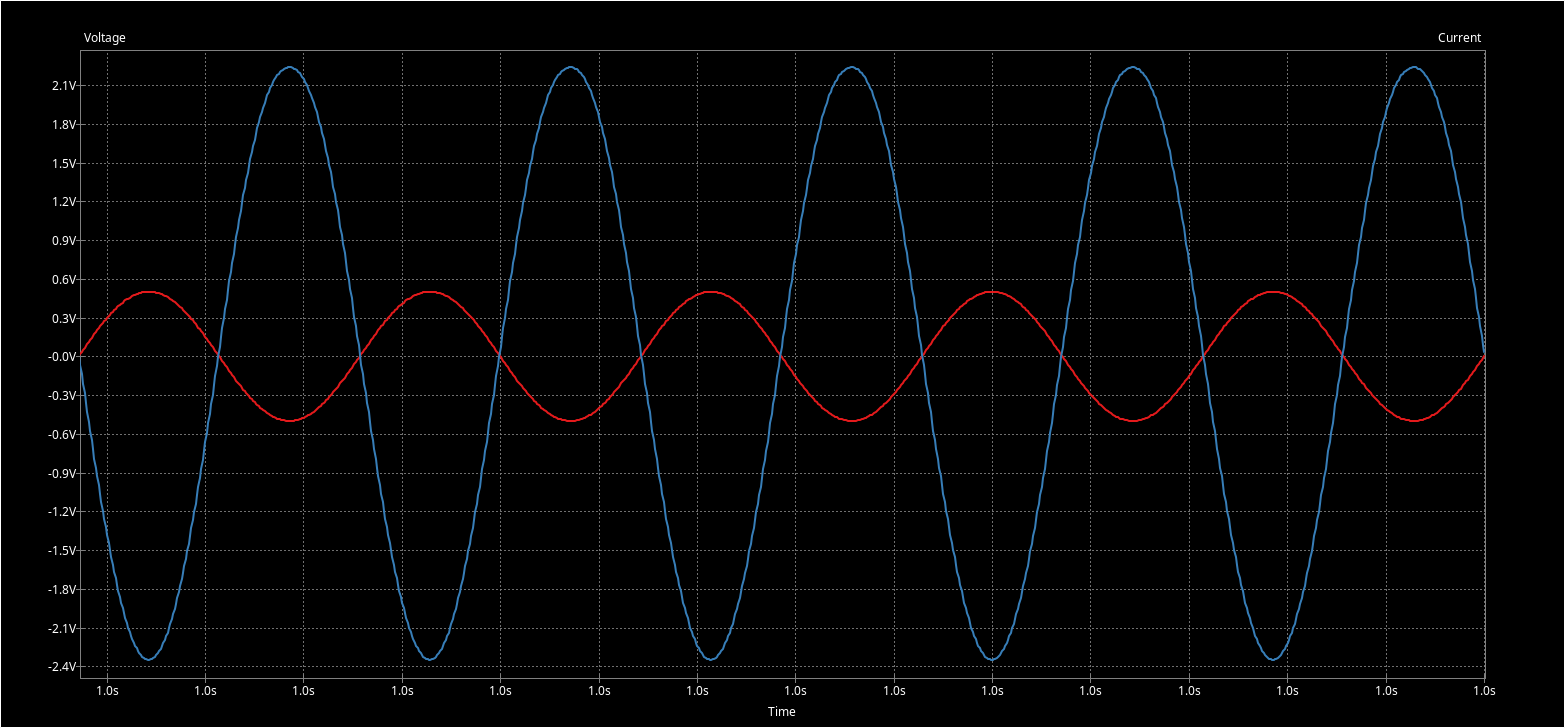
\includegraphics[scale=0.3]{imagenes/SimulacionCA.png}
\caption{$V_{in}$(Rojo) y $V_{out}$(Azul), simulados entre $1\second$ y $1,001\second$ segundos, en intervalos de $1\microsecond$}
\label{fig:SimulacionCA}
\end{figure}

\begin{figure}[!ht]
\centering
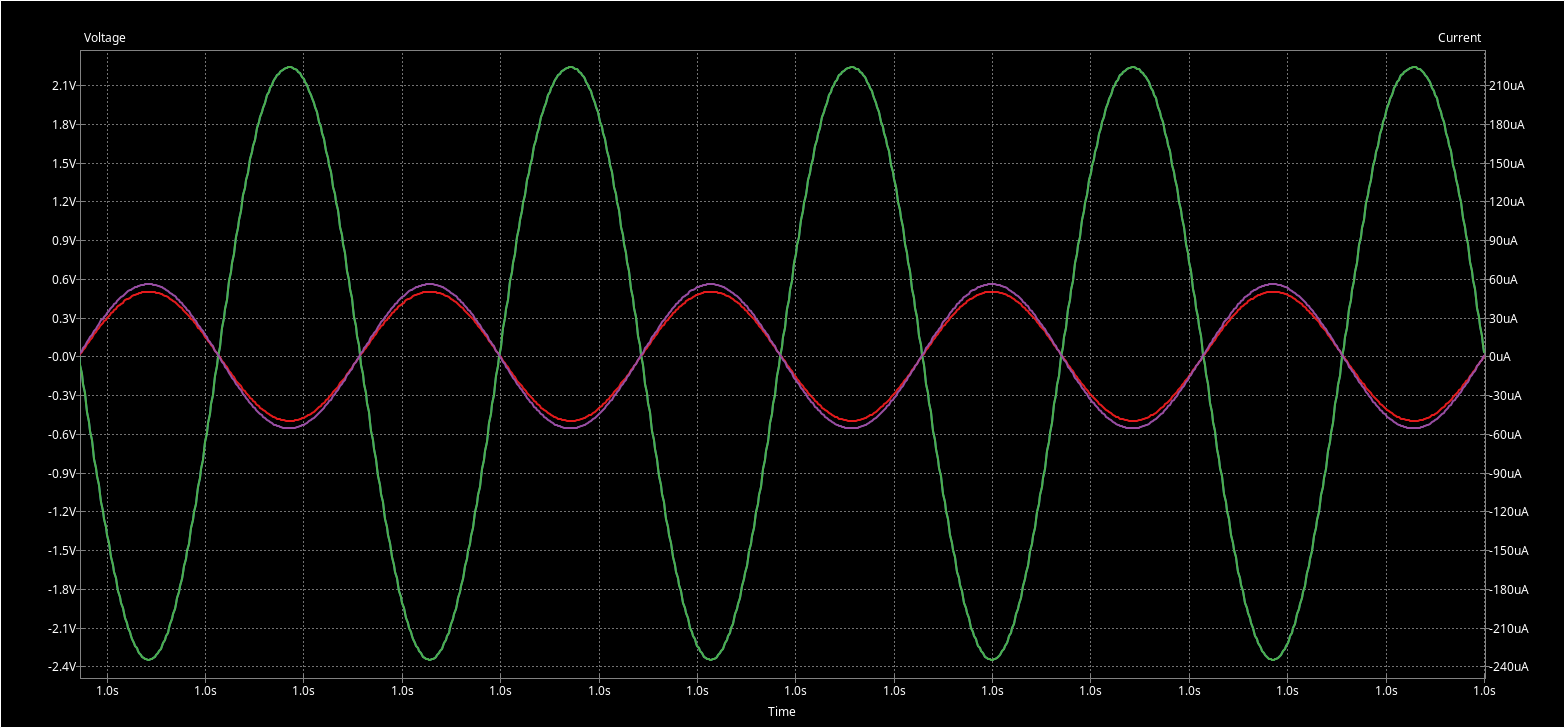
\includegraphics[scale=0.3]{imagenes/SimulacionCACorrientes.png}
\caption{Misma simulación que la figura \ref{fig:SimulacionCA}, añadidas $i_{in}$(Violeta) y $i_{out}$(Verde)}
\label{fig:SimulacionCACorrientes}
\end{figure}

\subsection{}

Poner un capacitor de desacople en paralelo con $R_3$ daría al circuito una mayor excursión, 
una mayor ganancia de tensión y una mejor transferencia de potencia. La excursión y la 
transferencia de potencia mejorar al no tener una perdida por la caída de tensión en $R_3$.
La mejora en la amplificación de tensión, viene dada por una reducción en la impedancia de
entrada, que causa que a igual tensión se tenga una mayor corriente de base.

\newpage
\section{Laboratorio}
\subsection{}

Tras implementar el circuito en protoboard se observó la señal que se muestra en la figura \ref{fig:1}.
Vemos que los valores pico a pico capturados nos muestran $V_{in} = 1,08\volt$ y $V_{out} = 4,35\volt$.
Con estos datos podemos calcular $A_V$ como se muestra en la ecuación \ref{ecu:AVMed}.

\begin{figure}[!ht]
\centering
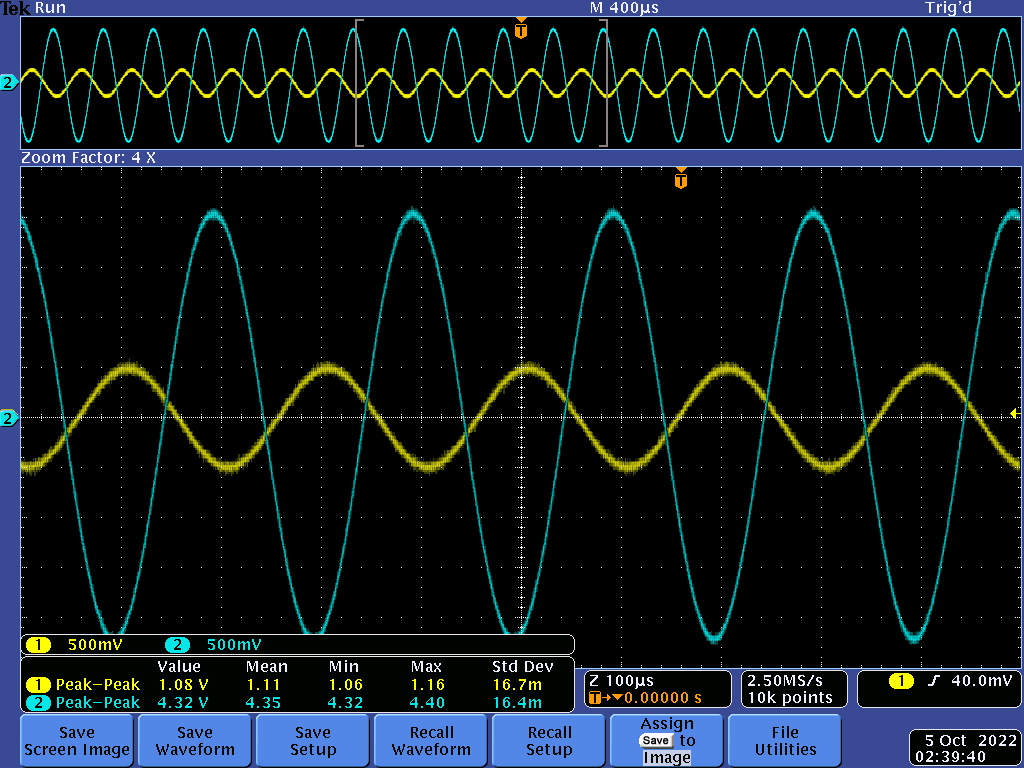
\includegraphics[scale=0.5]{imagenes/1.png}
\caption{$1,11\volt_{pp}$}
\label{fig:1}
\end{figure}

\begin{equation}
	A_V=
	\frac{
		-4,35\volt
	}{
		1,11\volt
	}\approx
	-3,919
\label{ecu:AVMed}
\end{equation}

Luego de incrementar la amplitud en un $20\%$ se observó una pequeña caída en la ganancia,
como se muestra en la ecuación \ref{ecu:AVMed2}, con datos de la figura \ref{fig:2}.

\begin{figure}[!ht]
\centering
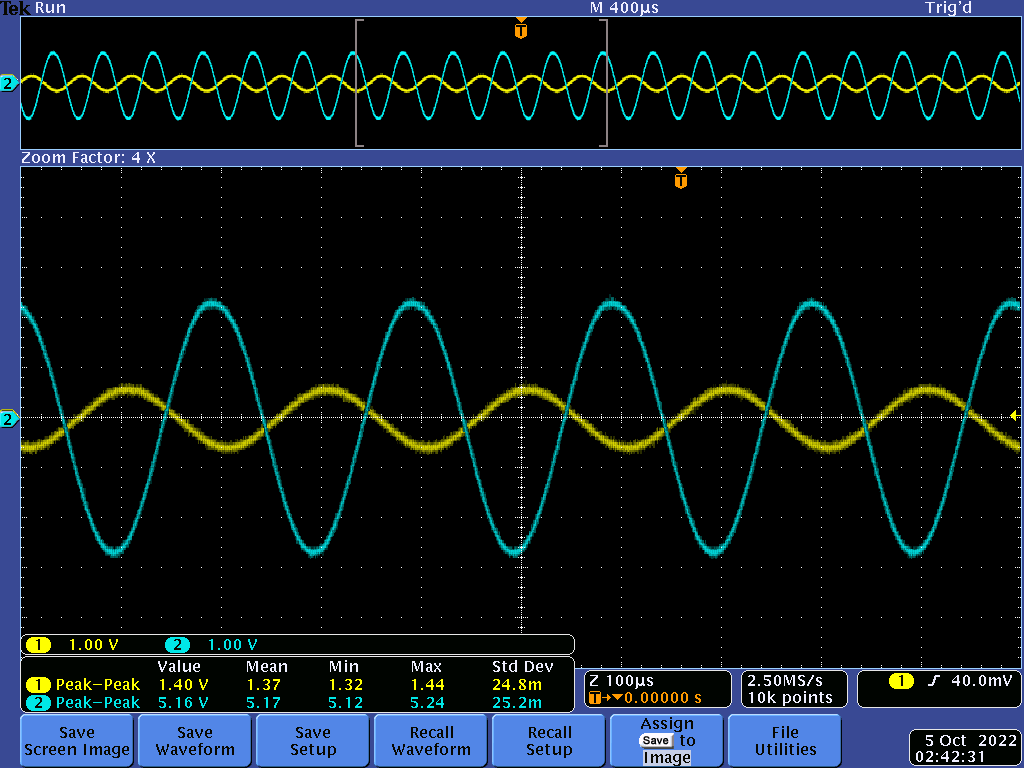
\includegraphics[scale=0.5]{imagenes/2.png}
\caption{$1,37\volt_{pp}$}
\label{fig:2}
\end{figure}

\begin{equation}
	A_V=
	\frac{
		-5,17\volt
	}{
		1,37\volt
	}\approx
	-3,774
\label{ecu:AVMed2}
\end{equation}

\newpage
Entre la figura \ref{fig:3} y la figura \ref{fig:12} se muestra un avance progresivo con 
pasos de aproximadamente $100\millivolt$, donde se busca el punto de recorte en cada sentido
de la señal.\\
Con aproximadamente $1,45\volt_{pp}$ en la entrada comienza a verse un recorte en el pico superior.
El recorte del pico superior se vuelve progresivamente mas notorio a medida que aumenta la amplitud
de entrada. No es hasta que la tensión de entrada alcanza una amplitud de aproximadamente $2,35\volt_{pp}$
que comienza a notarse el recorte inferior de la señal.

\begin{figure}[!ht]
\centering
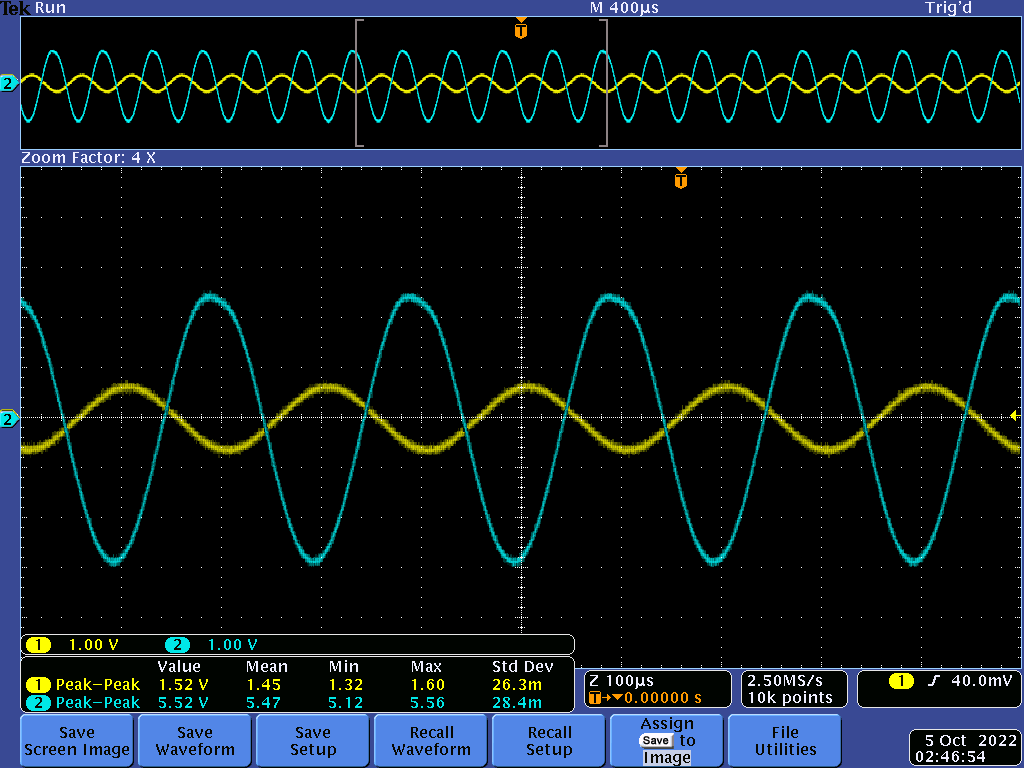
\includegraphics[scale=0.5]{imagenes/3.png}
\caption{$1,45\volt_{pp}$}
\label{fig:3}
\end{figure}

\begin{figure}[!ht]
\centering
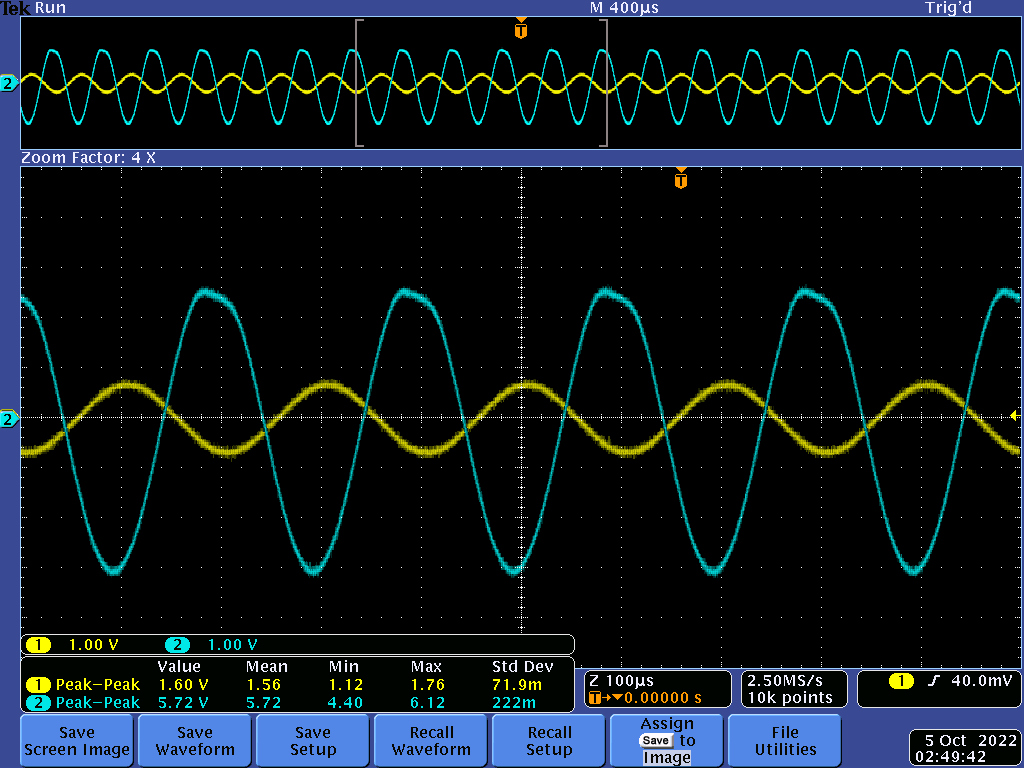
\includegraphics[scale=0.5]{imagenes/4.png}
\caption{$1,56\volt_{pp}$}
\label{fig:4}
\end{figure}

\begin{figure}[!ht]
\centering
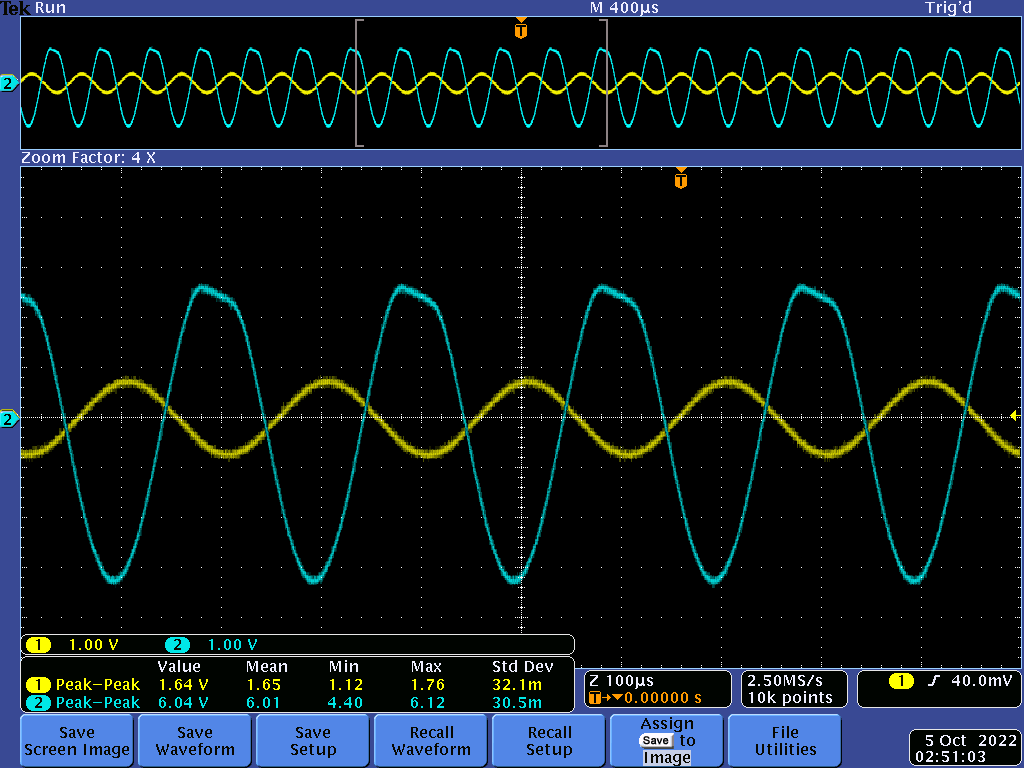
\includegraphics[scale=0.5]{imagenes/5.png}
\caption{$1,66\volt_{pp}$}
\label{fig:5}
\end{figure}

\begin{figure}[!ht]
\centering
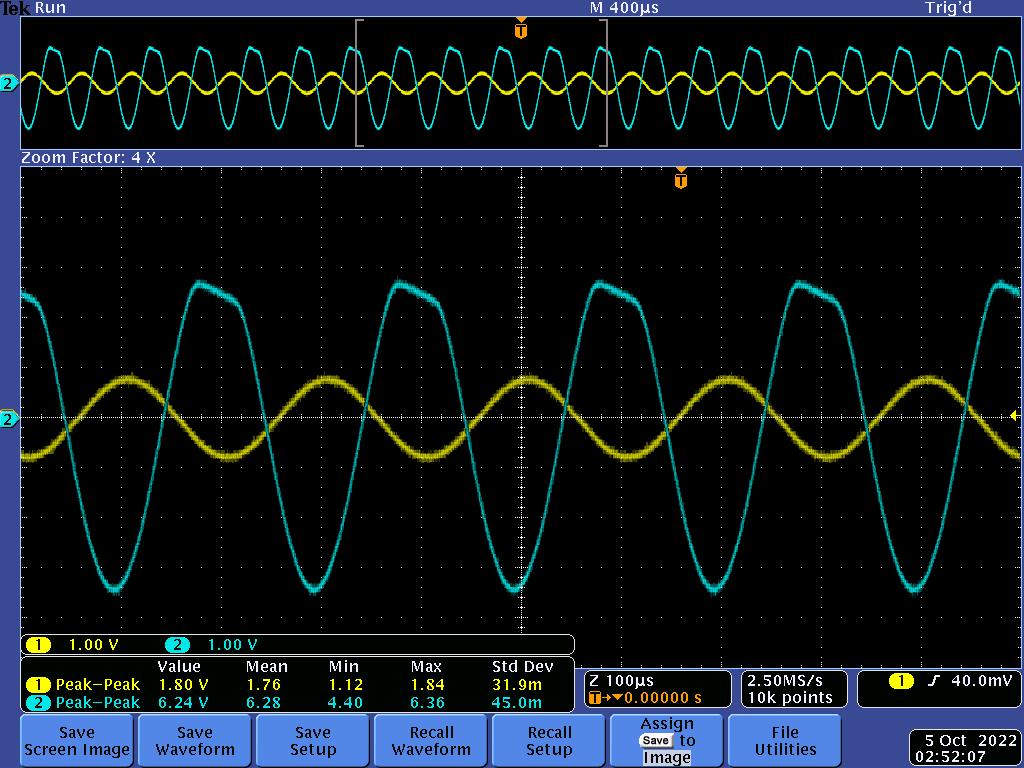
\includegraphics[scale=0.5]{imagenes/6.png}
\caption{$1,75\volt_{pp}$}
\label{fig:6}
\end{figure}

\begin{figure}[!ht]
\centering
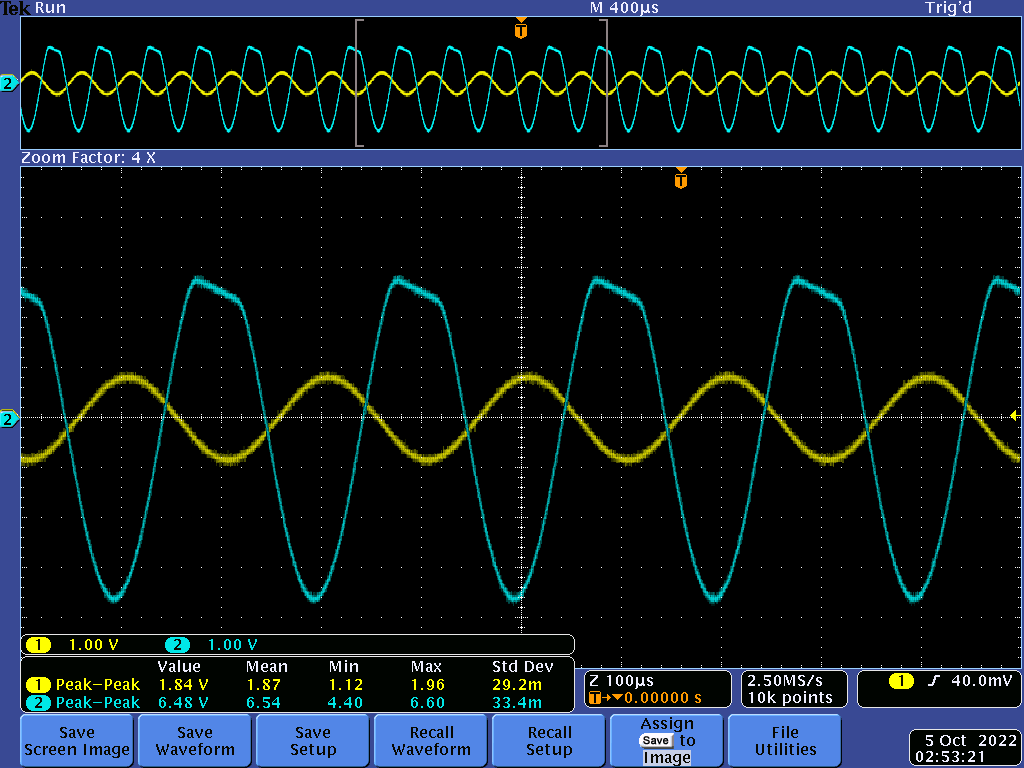
\includegraphics[scale=0.5]{imagenes/7.png}
\caption{$1,86\volt_{pp}$}
\label{fig:7}
\end{figure}

\begin{figure}[!ht]
\centering
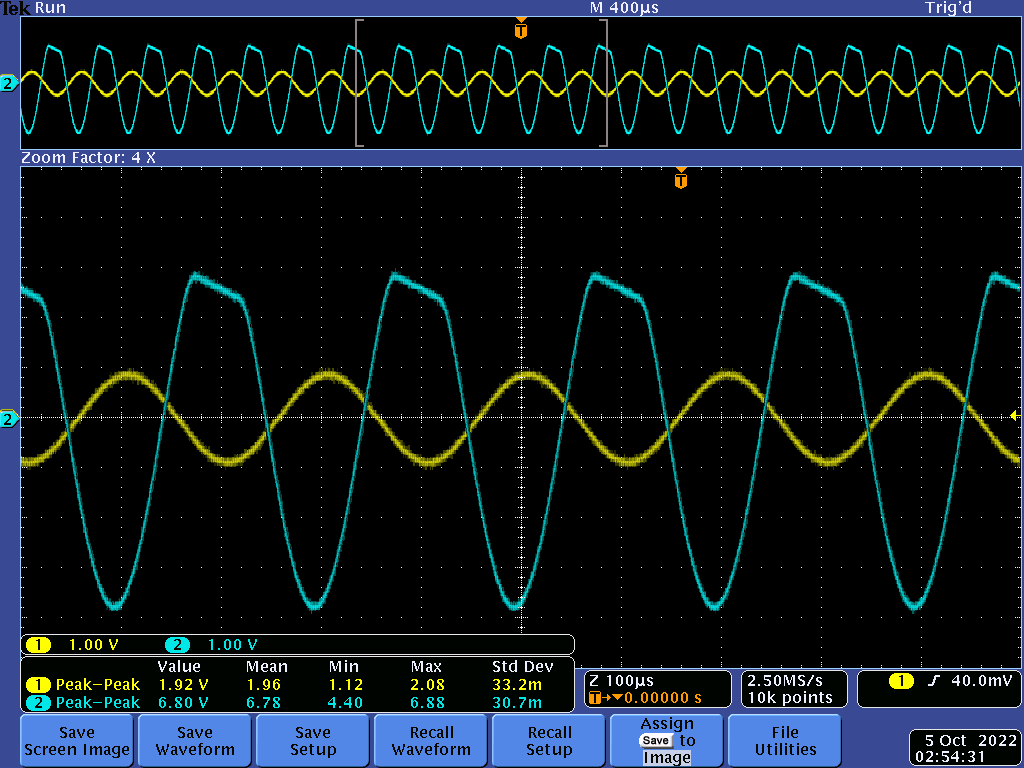
\includegraphics[scale=0.5]{imagenes/8.png}
\caption{$1,96\volt_{pp}$}
\label{fig:8}
\end{figure}

\begin{figure}[!ht]
\centering
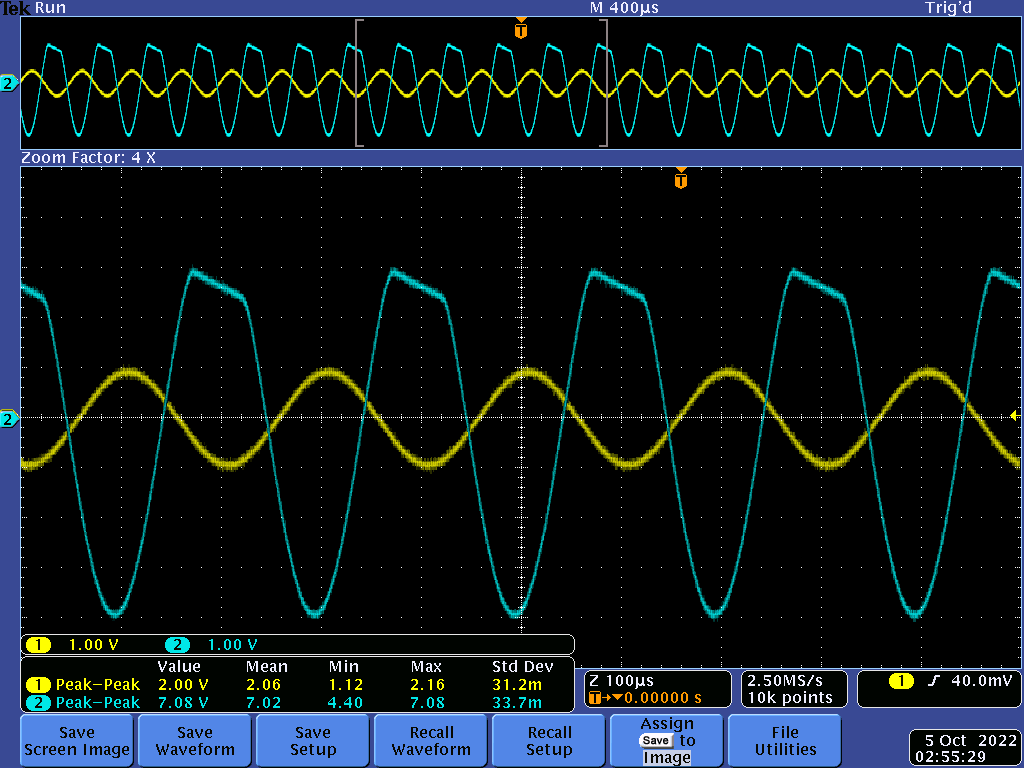
\includegraphics[scale=0.5]{imagenes/9.png}
\caption{$2,05\volt_{pp}$}
\label{fig:9}
\end{figure}

\begin{figure}[!ht]
\centering
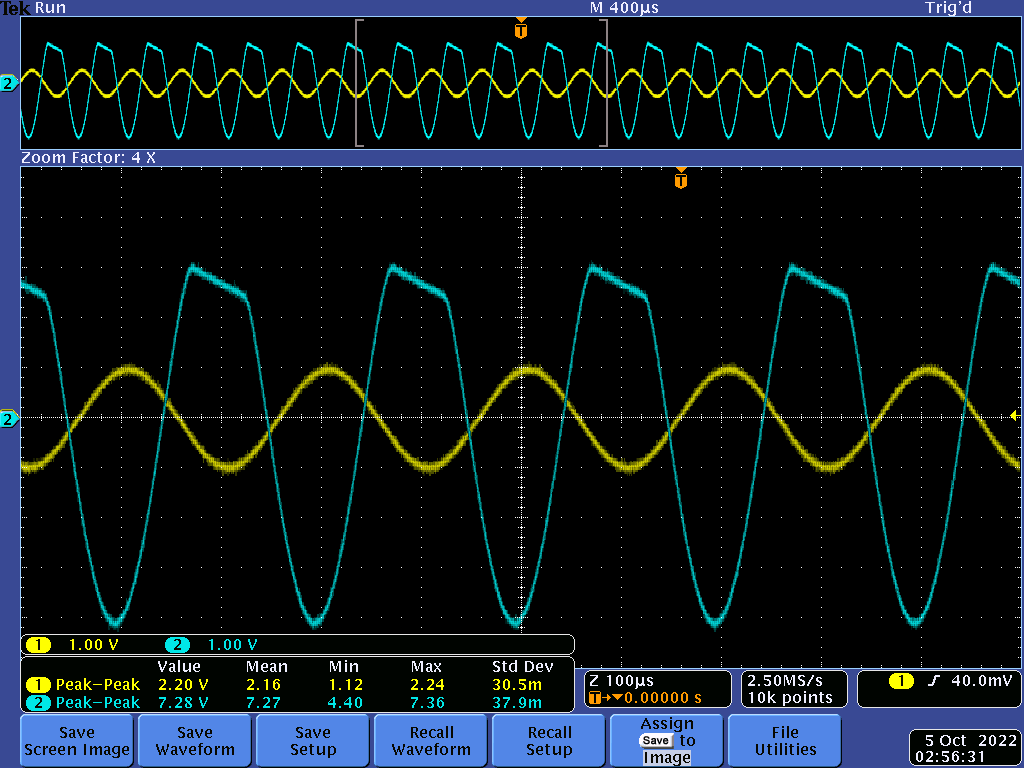
\includegraphics[scale=0.5]{imagenes/10.png}
\caption{$2,15\volt_{pp}$}
\label{fig:10}
\end{figure}

\begin{figure}[!ht]
\centering
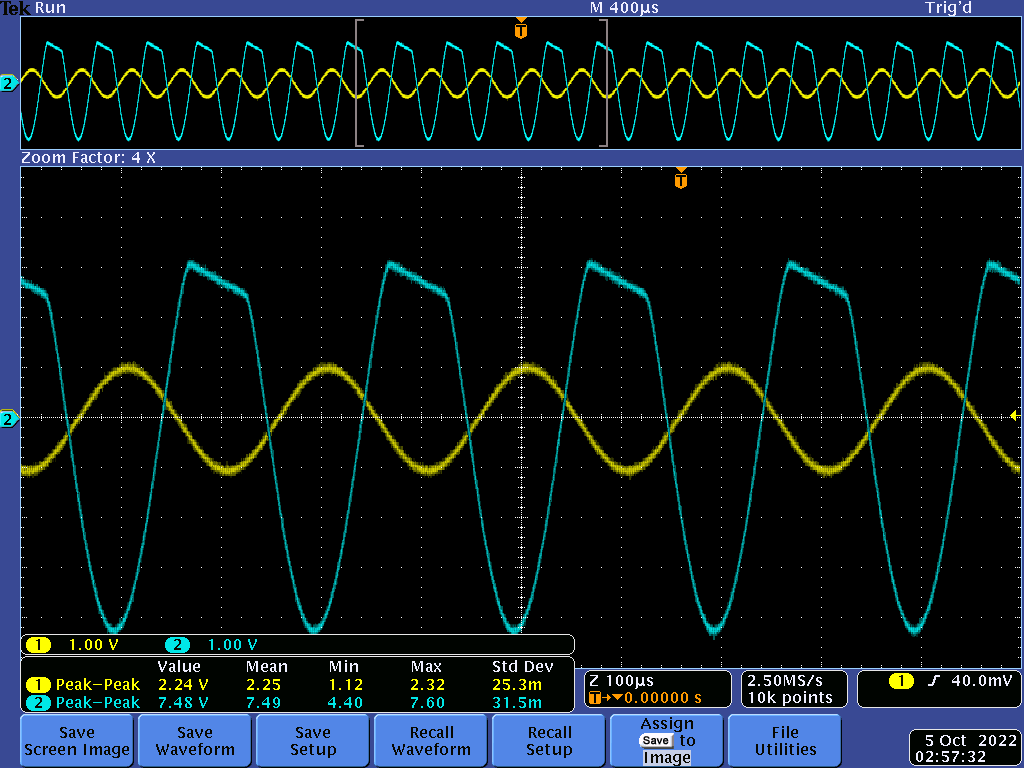
\includegraphics[scale=0.5]{imagenes/11.png}
\caption{$2,25\volt_{pp}$}
\label{fig:11}
\end{figure}

\begin{figure}[!ht]
\centering
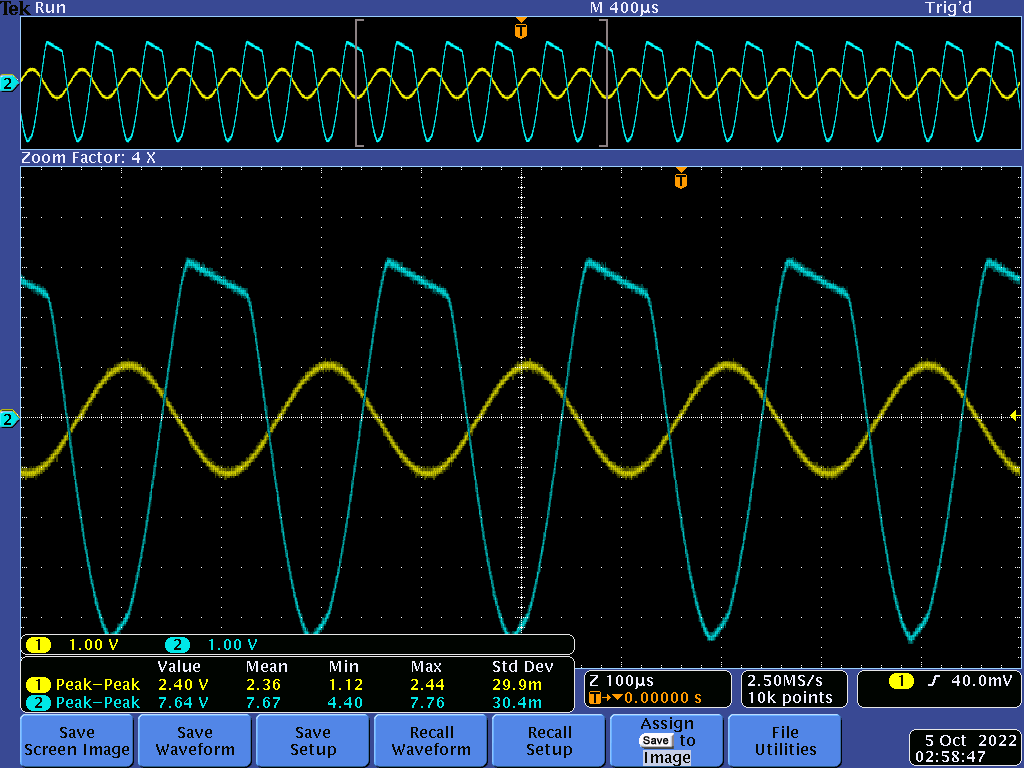
\includegraphics[scale=0.5]{imagenes/12.png}
\caption{$2,35\volt_{pp}$}
\label{fig:12}
\end{figure}

\clearpage
\subsection{}

Las mediciones obtenidas se muestran en la tabla \ref{tab:PuntoDeTrabajoMeida}.
Las medidas de corriente se realizaron a partir de medidas de tensión
$I_{CQ} = \frac{5,188\volt}{10\kiloohm}$ y
$I_{C\sim} = \frac{1,61\volt_{\sim}}{10\kiloohm}$.

\begin{table}[!ht]
	\begin{center}
		\begin{tabular}{| c | c | c |}
			\hline
			\textbf{Parámetro} & \textbf{Valor} & \textbf{Unidad}\\ 
			\hline
			{$I_{CQ}$} & {511,8} & {$\microampere$}\\
			\hline
			{$V_{CEQ}$} & {6,434} & {$\volt$}\\
			\hline
			{$I_{C\sim}$} & {161} & {$\microampere_{\sim}$}\\
			\hline
			{$V_{CE\sim}$} & {1,924} & {$\volt_{\sim}$}\\
			\hline
		\end{tabular}
	\end{center}
	\caption{Valores obtenidos mediante mediciones}
\label{tab:PuntoDeTrabajoMeida}
\end{table}

Para una comparativa general entre los datos calculados, simulados y medidos
se recompilaron todos valores, conocidos de las tres maneras
en la tabla \ref{tab:ComparativaFinal}.
El valor de $V_{CQ}$ medido se lo calcula a partir de $V_{CEQ}$, $I_{CQ}$ y $R_3$.

\begin{table}[!ht]
	\begin{center}
		\begin{tabular}{| c | c | c | c | c |}
			\hline
			\textbf{Parámetro} & \textbf{Valor calculado} & \textbf{Valor simulado} & \textbf{Valor medido} & \textbf{Unidad}\\ 
			\hline
			{$A_V$} & {-4,663}  & {-4,4744}& {-3,919} & {} \\
			\hline
			{$I_{CQ}$} & {369,2} & {494,684} & {511,8} & {$\microampere$}\\
			\hline
			{$V_{CQ}$} & {8,308} & {7,05317} & {6,9458} & {$\volt$}\\
			\hline
			{$V_{CEQ}$} & {7,93809} & {7,007591} & {6,434} & {$\volt$}\\
			\hline
		\end{tabular}
	\end{center}
	\caption{Punto de trabajo circuito \ref{circuito1}}
\label{tab:ComparativaFinal}
\end{table}

\newpage
\subsection{}

Para el análisis en frecuencia se tomaron las siguiente medidas mostradas entre la figura \ref{fig:23}
y la figura \ref{fig:18}

\begin{figure}[!ht]
\centering
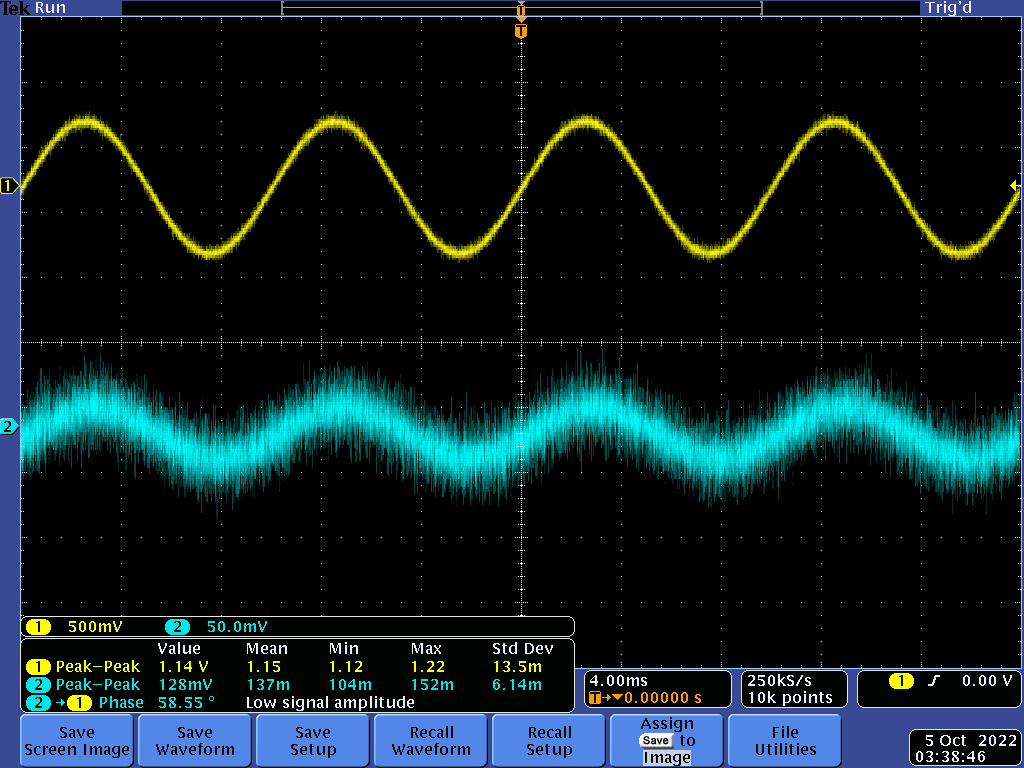
\includegraphics[scale=0.5]{imagenes/23.png}
\caption{$100\hertz$}
\label{fig:23}
\end{figure}

\begin{figure}[!ht]
\centering
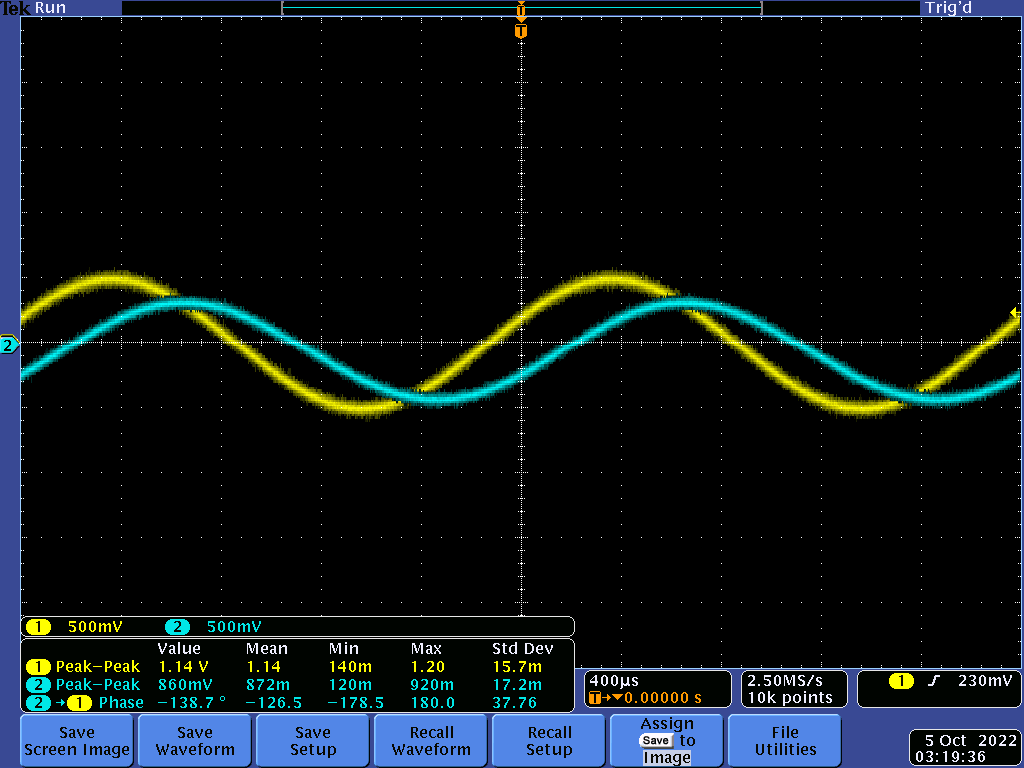
\includegraphics[scale=0.5]{imagenes/13.png}
\caption{$500\hertz$}
\label{fig:13}
\end{figure}

\begin{figure}[!ht]
\centering
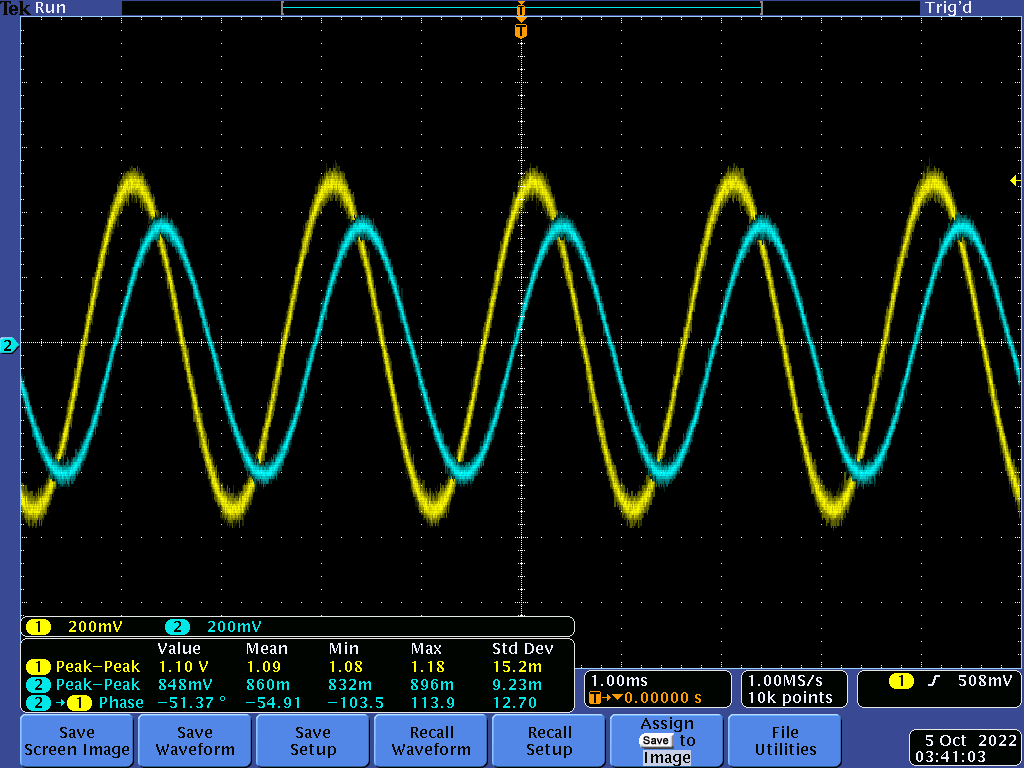
\includegraphics[scale=0.5]{imagenes/22.png}
\caption{$500\hertz$ Alternativa}
\label{fig:22}
\end{figure}

\begin{figure}[!ht]
\centering
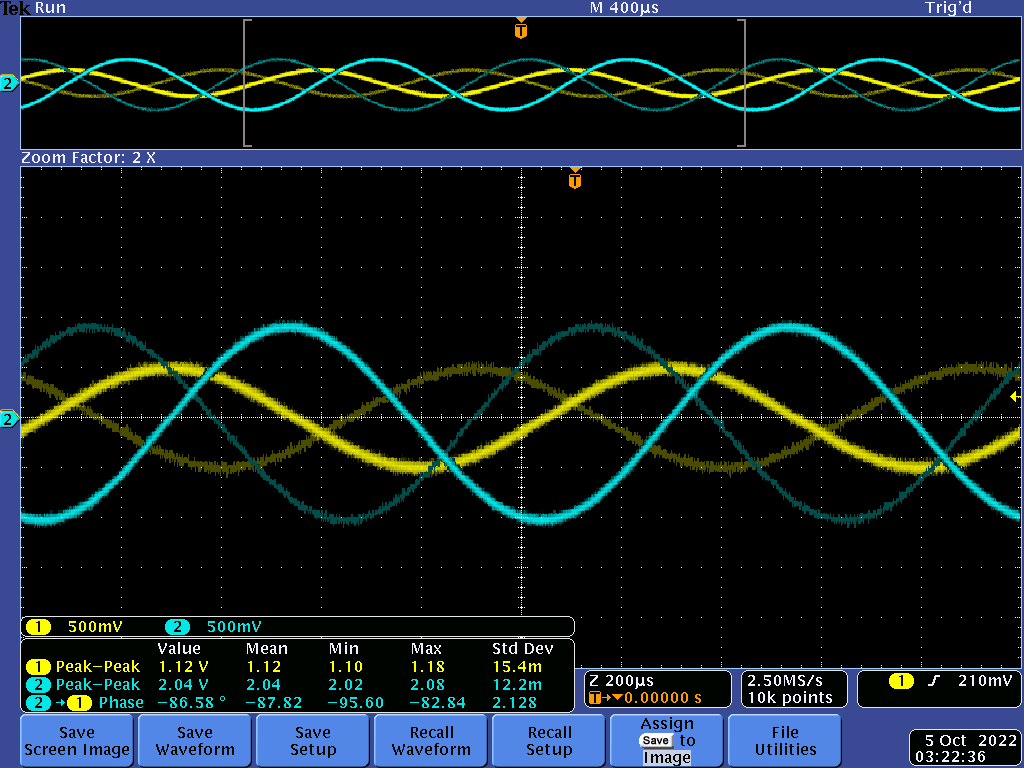
\includegraphics[scale=0.5]{imagenes/14.png}
\caption{$1\kilohertz$}
\label{fig:14}
\end{figure}

\begin{figure}[!ht]
\centering
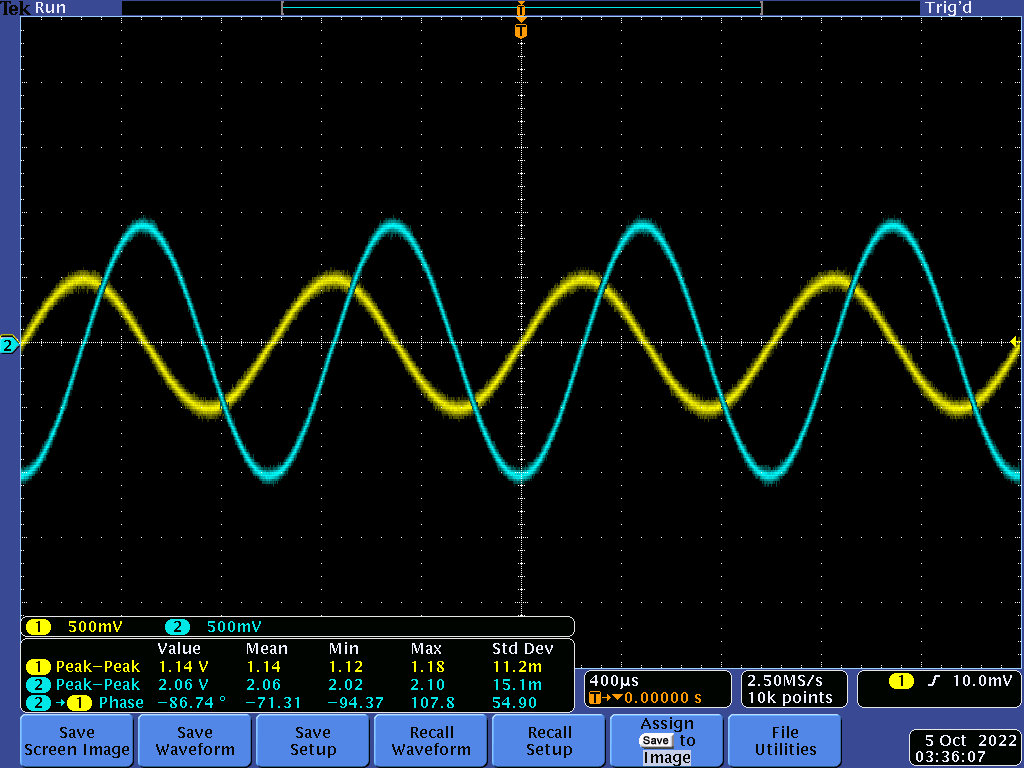
\includegraphics[scale=0.5]{imagenes/21.png}
\caption{$1\kilohertz$ Alternativa}
\label{fig:21}
\end{figure}

\begin{figure}[!ht]
\centering
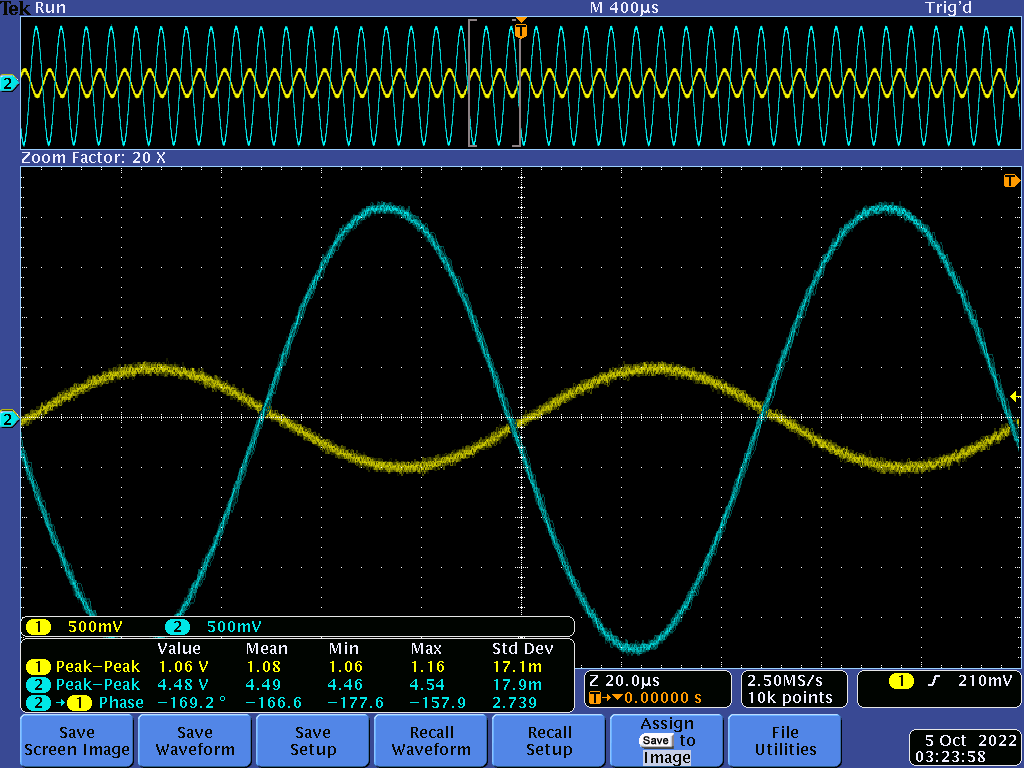
\includegraphics[scale=0.5]{imagenes/15.png}
\caption{$10\kilohertz$}
\label{fig:15}
\end{figure}

\begin{figure}[!ht]
\centering
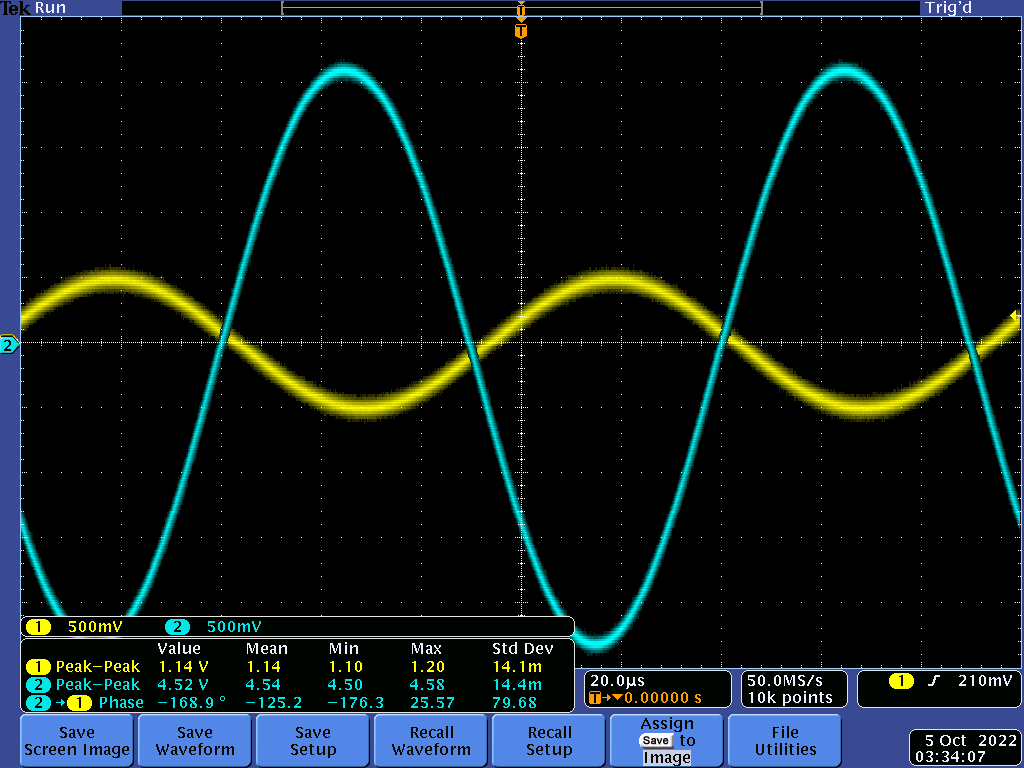
\includegraphics[scale=0.5]{imagenes/20.png}
\caption{$10\kilohertz$ Alternativa}
\label{fig:20}
\end{figure}

\begin{figure}[!ht]
\centering
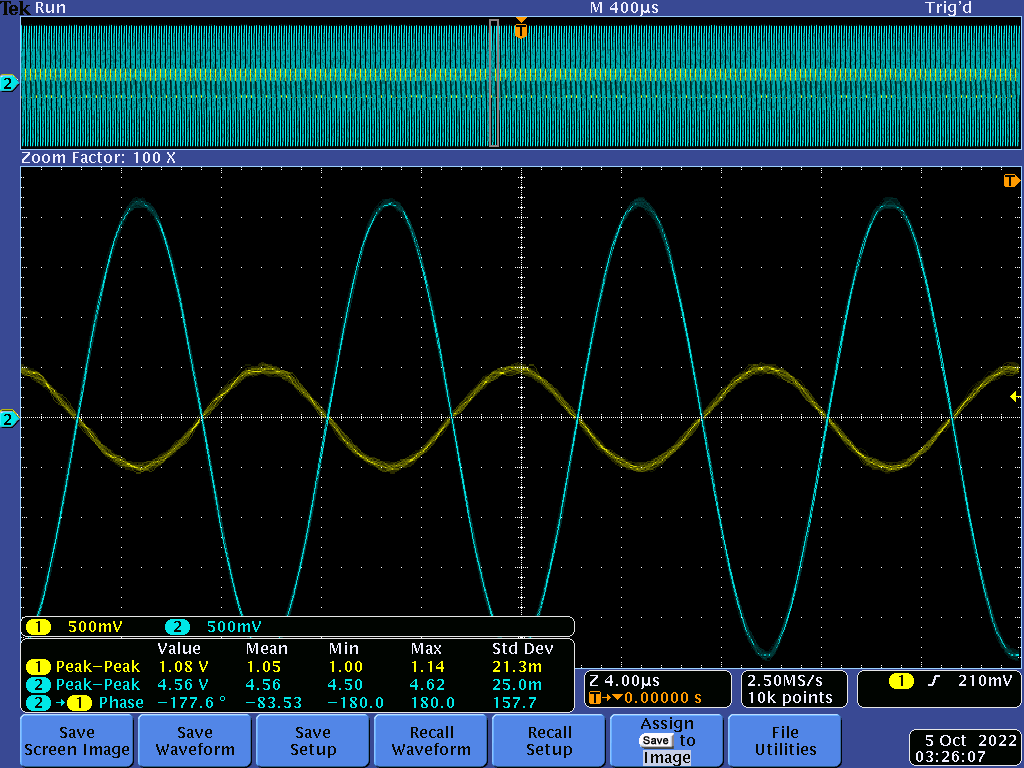
\includegraphics[scale=0.5]{imagenes/16.png}
\caption{$100\kilohertz$}
\label{fig:16}
\end{figure}

\begin{figure}[!ht]
\centering
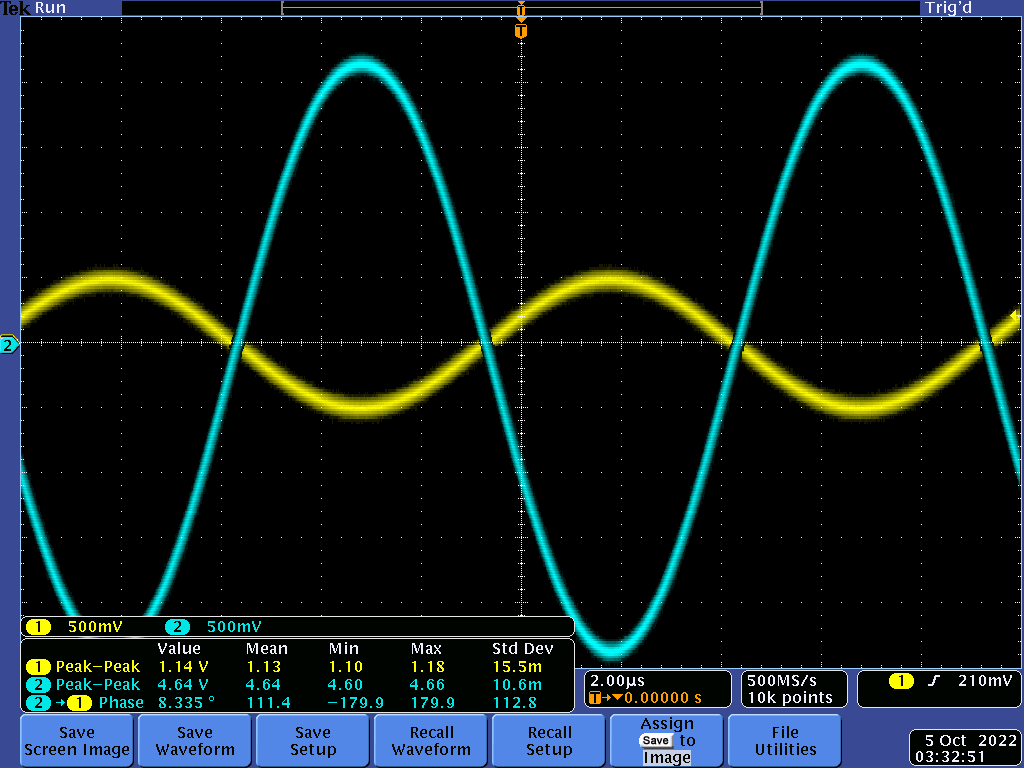
\includegraphics[scale=0.5]{imagenes/19.png}
\caption{$100\kilohertz$ Alternativa}
\label{fig:19}
\end{figure}

\begin{figure}[!ht]
\centering
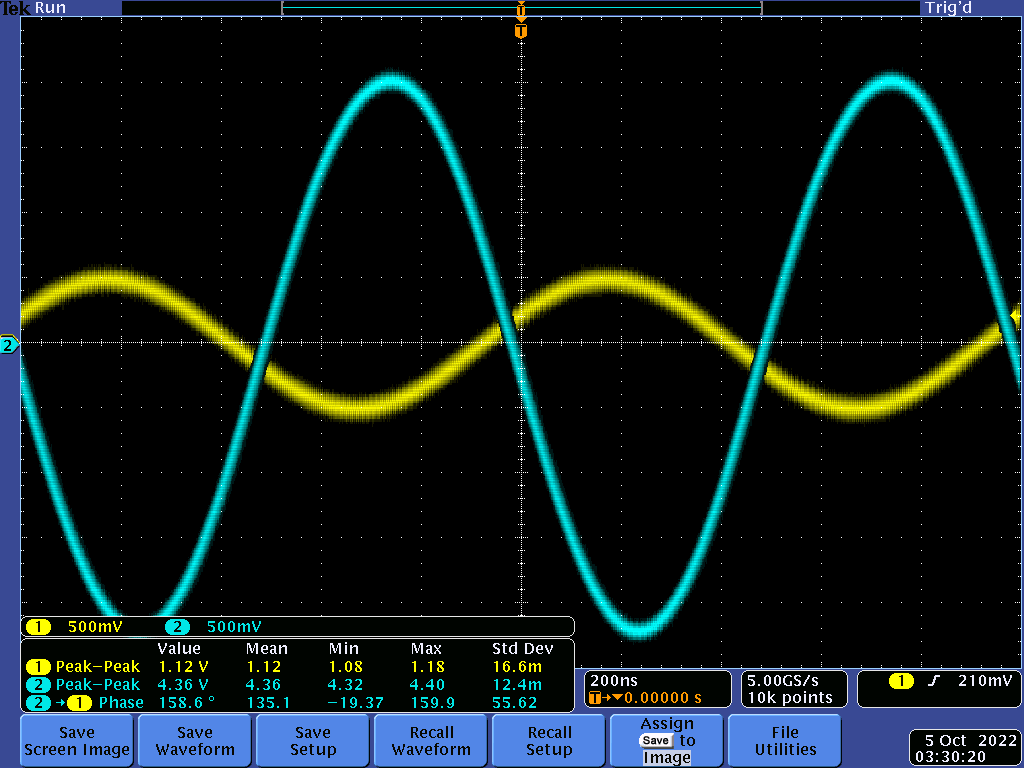
\includegraphics[scale=0.5]{imagenes/17.png}
\caption{$1\megahertz$}
\label{fig:17}
\end{figure}

\begin{figure}[!ht]
\centering
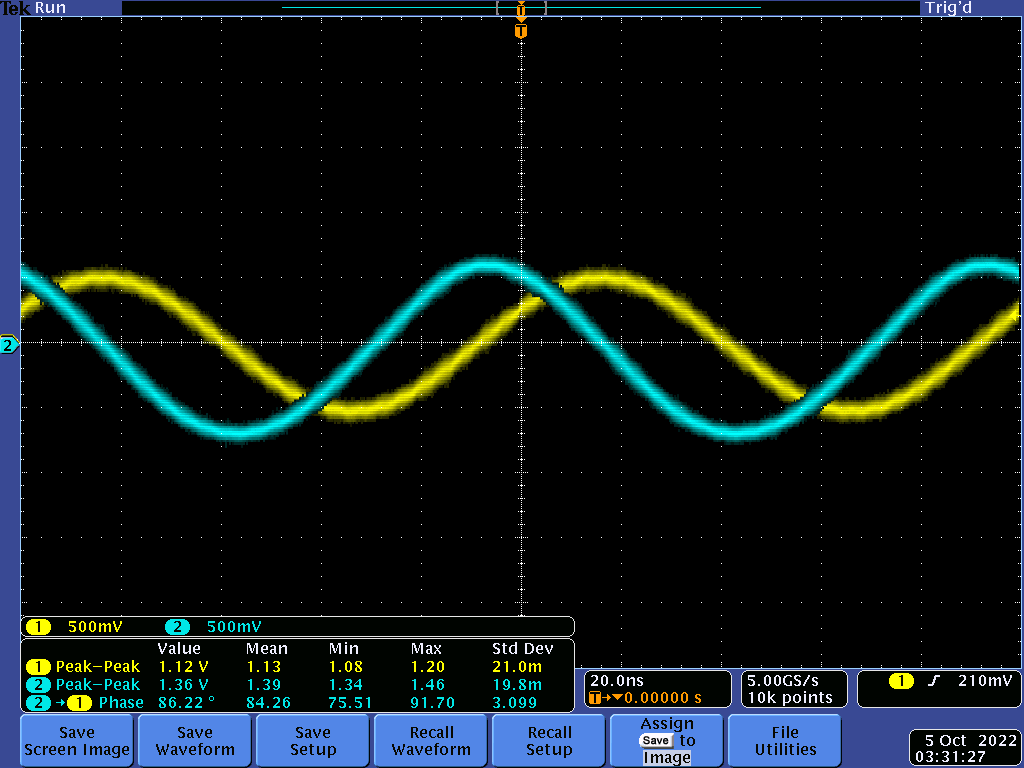
\includegraphics[scale=0.5]{imagenes/18.png}
\caption{$10\megahertz$}
\label{fig:18}
\end{figure}

\clearpage
De estas imágenes se calcularon las ganancias correspondientes en db,
las que se muestran recompiladas en la tabla \ref{tab:RespuestaEnFrecuencia}.

\begin{table}[!ht]
	\begin{center}
		\begin{tabular}{| c | c | c |}
			\hline
			\textbf{Frecuencia} & \textbf{$A_V[db]$} & \textbf{$\phi[\degree]$}\\ 
			\hline
			{100\hertz} & {-19,6}  & {0}\\
			\hline
			{500\hertz} & {-2,5}  & {45}\\
			\hline
			{500\hertz} & {-2,43}  & {45}\\
			\hline
			{1\kilohertz} & {4,95}  & {90}\\
			\hline
			{1\kilohertz} & {5,2}  & {90}\\
			\hline
			{10\kilohertz} & {12,2}  & {-166}\\
			\hline
			{10\kilohertz} & {12}  & {-168}\\
			\hline
			{100\kilohertz} & {12,1}  & {180}\\
			\hline
			{100\kilohertz} & {12,6}  & {180}\\
			\hline
			{1\megahertz} & {11,58}  & {135}\\
			\hline
			{10\megahertz} & {1,7}  & {-90}\\
			\hline
		\end{tabular}
	\end{center}
\caption{Valores de respuesta en frecuencia obtenidos en el laboratorio}
\label{tab:RespuestaEnFrecuencia}
\end{table}

A partir de estos valores se construyeron los diagramas de modulo 
(figura \ref{fig:DiagramDeModulo})
y fase (figura \ref{fig:DiagramDeFase}).

\begin{figure}[!ht]
	\begin{center}
		\begin{tikzpicture}
				\begin{semilogxaxis}[
					 enlargelimits=true,
					 ymajorgrids=true,
					 xmajorgrids=true,
					 grid style=dashed,
				]
				\addplot+[
					 scatter,
					 mark=*,
					 mark size=2pt]
					 table[blue]
				{
					A	B	
					100	-19.6	
					500	-2.5
					500	-2.43
					1000	4.95
					1000	5.2
					10000	12.2
					10000	12	
					100000	12.1
					100000	12.6
					1000000	11.58
					10000000	1.7	
				};
				\end{semilogxaxis}
		\end{tikzpicture}
	\end{center}
\caption{Diagrama de modulo}
\label{fig:DiagramDeModulo}
\end{figure}

\begin{figure}[!ht]
	\begin{center}
		\begin{tikzpicture}
			\begin{semilogxaxis}[
				 enlargelimits=true,
				 ymajorgrids=true,
				 xmajorgrids=true,
				 grid style=dashed,
			]
			\addplot+[
				 scatter,
				 mark=*,
				 mark size=2pt]
				 table[red]
			{
				A	B	
				100	0
				500	-45
				500	-45
				1000	-90
				1000	-90
				10000	-166
				10000	-168
				100000	180
				100000	180
				1000000	135
				10000000	90
			};
			\end{semilogxaxis}
		\end{tikzpicture}
	\end{center}
\caption{Diagrama de fase}
\label{fig:DiagramDeFase}
\end{figure}

Los gráficos obtenidos experimentalmente, asemejan la silueta de los simulados (figura \ref{fig:ModuloYFase}).
Aunque los valores de modulo no coinciden en ningún punto, los de fase están
bastante acertados, y el comportamiento de pasa banda se aprecia en ambos.

\begin{figure}[!ht]
\centering
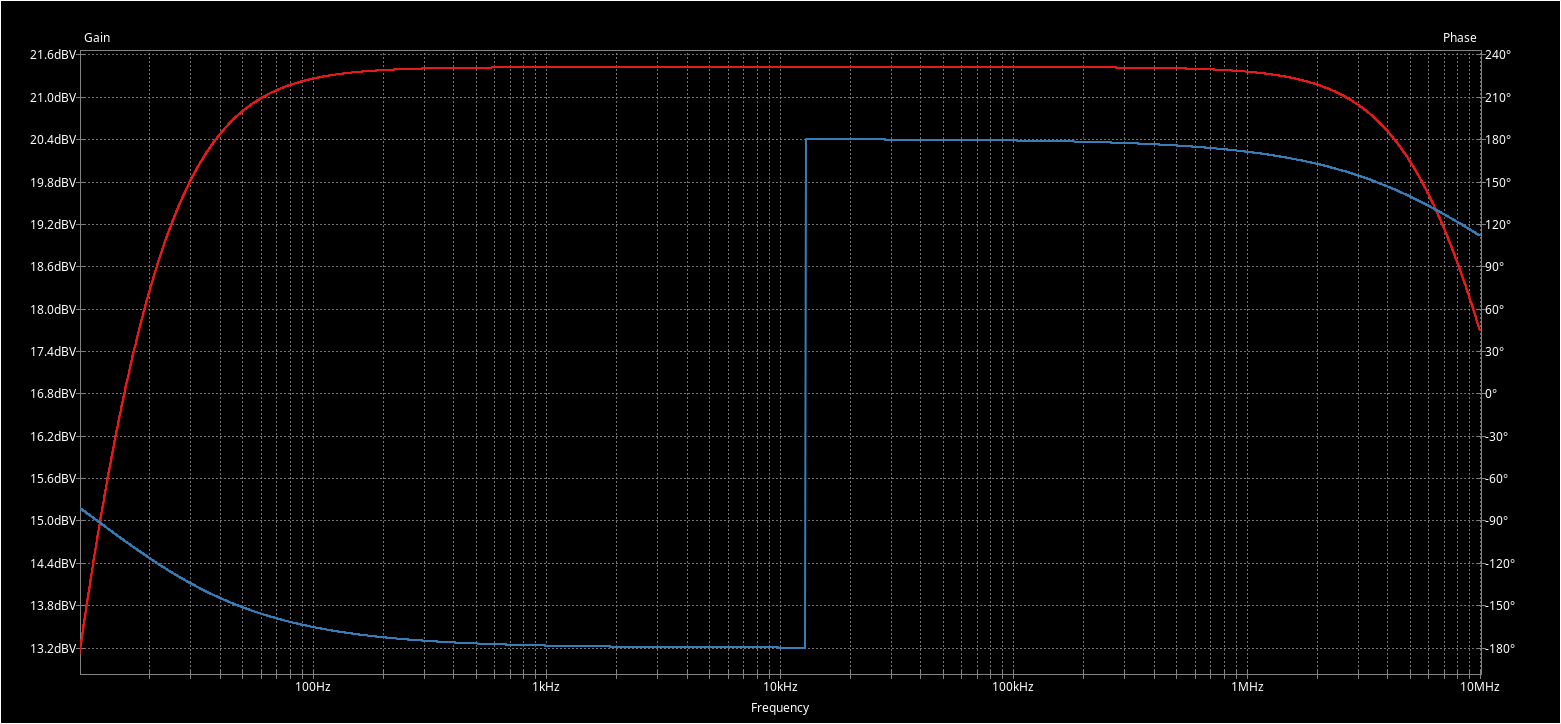
\includegraphics[scale=0.3]{imagenes/ModuloYFase.png}
\caption{Diagrama de modulo y fase simulado}
\label{fig:ModuloYFase}
\end{figure}

\clearpage
\section{Conclusiones}

Se obtuvieron resultados coherentes entre la practica, la simulación y el calculo analítico.
Los resultados no fueron idénticos en cada ámbito, esto es esperable ya que los cálculos fueron
realizados mediante un modelo simplificado, y la simulación es incapaz de ponderar todos los
fenómenos de la naturaleza.\\
Una de las mayores dificultades fue obtener una medición confiable de la diferencia de fase
entre dos señales, al ser ambas sinusoidales fue posible estimar la diferencia de forma 
intuitiva, pero realizar mediciones de ese estilo sobre una señal mas compleja podría traer 
múltiples desafíos.\\
Este amplificador tiene un ancho de banda que parece ir desde aproximadamente $1\kilohertz$,
hasta $1\megahertz$, dentro de este ancho de banda la ganancia es bastante estable, y la fase
se ve consistentemente invertida. Sumado a eso al ser una configuración polarizada en la zona
activa del transistor, tiene un comportamiento muy lineal y no presenta casi distorsión.\\
Por su baja distorsión podría ser usado para audio, aunque solo serviría como un amplificador
de altos. Por su ancho de banda podría utilizarse como un amplificador de radiofrecuencia,
con aplicación marítima de muy baja frecuencia o en AM, aunque su aplicación estaría limitada
a preamplificar por su baja potencia.

\end{document}
